%Version 3.1 December 2024
% See section 11 of the User Manual for version history
%
%%%%%%%%%%%%%%%%%%%%%%%%%%%%%%%%%%%%%%%%%%%%%%%%%%%%%%%%%%%%%%%%%%%%%%
%%                                                                 %%
%% Please do not use \input{...} to include other tex files.       %%
%% Submit your LaTeX manuscript as one .tex document.              %%
%%                                                                 %%
%% All additional figures and files should be attached             %%
%% separately and not embedded in the \TeX\ document itself.       %%
%%                                                                 %%
%%%%%%%%%%%%%%%%%%%%%%%%%%%%%%%%%%%%%%%%%%%%%%%%%%%%%%%%%%%%%%%%%%%%%

%%\documentclass[referee,sn-basic]{sn-jnl}% referee option is meant for double line spacing

%%=======================================================%%
%% to print line numbers in the margin use lineno option %%
%%=======================================================%%

%%\documentclass[lineno,pdflatex,sn-basic]{sn-jnl}% Basic Springer Nature Reference Style/Chemistry Reference Style

%%=========================================================================================%%
%% the documentclass is set to pdflatex as default. You can delete it if not appropriate.  %%
%%=========================================================================================%%

%%\documentclass[sn-basic]{sn-jnl}% Basic Springer Nature Reference Style/Chemistry Reference Style

%%Note: the following reference styles support Namedate and Numbered referencing. By default the style follows the most common style. To switch between the options you can add or remove “Numbered” in the optional parenthesis. 
%%The option is available for: sn-basic.bst, sn-chicago.bst%  
 
%%\documentclass[pdflatex,sn-nature]{sn-jnl}% Style for submissions to Nature Portfolio journals
%%\documentclass[pdflatex,sn-basic]{sn-jnl}% Basic Springer Nature Reference Style/Chemistry Reference Style
\documentclass[referee,lineno,pdflatex,sn-basic]{sn-jnl}% Basic Springer Nature reference style; double spacing and line numbers (journal requirement)
%%\documentclass[pdflatex,sn-mathphys-ay]{sn-jnl}% Math and Physical Sciences Author Year Reference Style
%%\documentclass[pdflatex,sn-aps]{sn-jnl}% American Physical Society (APS) Reference Style
%%\documentclass[pdflatex,sn-vancouver-num]{sn-jnl}% Vancouver Numbered Reference Style
%%\documentclass[pdflatex,sn-vancouver-ay]{sn-jnl}% Vancouver Author Year Reference Style
%%\documentclass[pdflatex,sn-apa]{sn-jnl}% APA Reference Style
%%\documentclass[pdflatex,sn-chicago]{sn-jnl}% Chicago-based Humanities Reference Style

%%%% Standard Packages
%%<additional latex packages if required can be included here>

\usepackage{graphicx}%
\usepackage{multirow}%
\usepackage{amsmath,amssymb,amsfonts}%
\usepackage{booktabs,tabularx,array,multirow}
\usepackage{amsthm}%
\usepackage{mathrsfs}%
\usepackage[title]{appendix}%
\usepackage{xcolor}%
\usepackage{textcomp}%
\usepackage{manyfoot}%
\usepackage{booktabs}%
\usepackage{algorithm}%
\usepackage{algorithmicx}%
\usepackage{algpseudocode}%
\usepackage{listings}%
\usepackage{booktabs}%
\usepackage{graphicx}%
\usepackage{tikz}
\usetikzlibrary{mindmap,trees,shadows}
%%%%

%%%%%=============================================================================%%%%
%%%%  Remarks: This template is provided to aid authors with the preparation
%%%%  of original research articles intended for submission to journals published 
%%%%  by Springer Nature. The guidance has been prepared in partnership with 
%%%%  production teams to conform to Springer Nature technical requirements. 
%%%%  Editorial and presentation requirements differ among journal portfolios and 
%%%%  research disciplines. You may find sections in this template are irrelevant 
%%%%  to your work and are empowered to omit any such section if allowed by the 
%%%%  journal you intend to submit to. The submission guidelines and policies 
%%%%  of the journal take precedence. A detailed User Manual is available in the 
%%%%  template package for technical guidance.
%%%%%=============================================================================%%%%

%% as per the requirement new theorem styles can be included as shown below
\theoremstyle{thmstyleone}%
\newtheorem{theorem}{Theorem}%  meant for continuous numbers
%%\newtheorem{theorem}{Theorem}[section]% meant for sectionwise numbers
%% optional argument [theorem] produces theorem numbering sequence instead of independent numbers for Proposition
\newtheorem{proposition}[theorem]{Proposition}% 
%%\newtheorem{proposition}{Proposition}% to get separate numbers for theorem and proposition etc.

\theoremstyle{thmstyletwo}%
\newtheorem{example}{Example}%
\newtheorem{remark}{Remark}%

\theoremstyle{thmstylethree}%
\newtheorem{definition}{Definition}%

\raggedbottom
%%\unnumbered% uncomment this for unnumbered level heads

\hypersetup{hypertexnames=false}
\begin{document}

\title[HANFIS: Evidence-Based Dynamic Risk Scoring for Cloud-Native Kubernetes]{HANFIS: A Hierarchical Adaptive Neuro-Fuzzy Inference System for Evidence-Based Dynamic Cybersecurity Risk Scoring in Cloud-Native Kubernetes Deployments}

%%=============================================================%%
%% GivenName	-> \fnm{Joergen W.}
%% Particle	-> \spfx{van der} -> surname prefix
%% FamilyName	-> \sur{Ploeg}
%% Suffix	-> \sfx{IV}
%% \author*[1,2]{\fnm{Joergen W.} \spfx{van der} \sur{Ploeg} 
%%  \sfx{IV}}\email{iauthor@gmail.com}
%%=============================================================%%

\author*[1]{\fnm{Mohammad Hafiz} \sur{Hersyah}}\email{mohammadhafizhersyah02@it.unand.ac.id}

\author[2]{\fnm{Derisma} \sur{Derisma}}\email{derisma@it.unand.ac.id}
 

\author[1]{\fnm{Budi} \sur{Rahmadya}}\email{budi-r@it.unand.ac.id}


\affil*[1]{\orgdiv{Computer Engineering Department}, \orgname{Andalas University}, \orgaddress{\street{Kampus Limau Manis Street}, \city{Padang}, \postcode{25162}, \state{West Sumatera}, \country{Indonesia}}}

\affil[2]{\orgdiv{Informatics Department}, \orgname{Andalas University}, \orgaddress{\street{Kampus Limau Manis Street}, \city{Padang}, \postcode{25162}, \state{West Sumatera}, \country{Indonesia}}}

 

%%==================================%%
%% Sample for unstructured abstract %%
%%==================================%%

\abstract{Static, expert-weighted fuzzy risk scores go stale between elicitations, while a flat Adaptive Neuro-Fuzzy Inference System (ANFIS) over seven risk inputs requires 128 rules and 1{,}052 parameters. We propose a hierarchical ANFIS (HANFIS) that separates vulnerability and environmental reasoning before an integration tier adds threat intelligence, reducing the model to 34 rules and 176 parameters (73.4\% and 83.3\% fewer). We build a temporal exploitability-exposure target from sealed weekly Exploit Prediction Scoring System (EPSS) and Known Exploited Vulnerabilities (KEV) snapshots for 120 container images (6{,}357 asset-weeks), evaluated with grouped, embargoed splits. A 4-week persistence baseline lowers mean squared error relative to climatology by 97\%; a single Common Vulnerability Scoring System (CVSS) score, by 22\%. Under a protocol frozen before training, HANFIS reduces mean squared error by 96.7\% against CVSS, 69.6\% against a linear model and 66.5\% against a parameter-matched flat ANFIS (95\% bootstrap intervals excluding zero), but is not distinguishable from persistence. Post hoc analyses qualify these gains. Exact Shapley attribution puts 78.9\% on exploitability and the KEV indicator, ingredients of the label, and without them HANFIS has no skill over CVSS (skill $-0.14$, interval $-0.34$ to $0.05$). A four-parameter formula of those two inputs, $100\max(x_2,0.1\,x_7)$, has a lower error than HANFIS at four weeks (skill $-0.53$, interval $-1.44$ to $-0.21$); the gap narrows at longer horizons only through weeks around an EPSS model change. In a pre-registered forward evaluation, the formula beat persistence and HANFIS did not beat the formula. The data cannot show whether environmental context helps.}

%%================================%%
%% Sample for structured abstract %%
%%================================%%

% \abstract{\textbf{Purpose:} The abstract serves both as a general introduction to the topic and as a brief, non-technical summary of the main results and their implications. The abstract must not include subheadings (unless expressly permitted in the journal's Instructions to Authors), equations or citations. As a guide the abstract should not exceed 200 words. Most journals do not set a hard limit however authors are advised to check the author instructions for the journal they are submitting to.
% 
% \textbf{Methods:} The abstract serves both as a general introduction to the topic and as a brief, non-technical summary of the main results and their implications. The abstract must not include subheadings (unless expressly permitted in the journal's Instructions to Authors), equations or citations. As a guide the abstract should not exceed 200 words. Most journals do not set a hard limit however authors are advised to check the author instructions for the journal they are submitting to.
% 
% \textbf{Results:} The abstract serves both as a general introduction to the topic and as a brief, non-technical summary of the main results and their implications. The abstract must not include subheadings (unless expressly permitted in the journal's Instructions to Authors), equations or citations. As a guide the abstract should not exceed 200 words. Most journals do not set a hard limit however authors are advised to check the author instructions for the journal they are submitting to.
% 
% \textbf{Conclusion:} The abstract serves both as a general introduction to the topic and as a brief, non-technical summary of the main results and their implications. The abstract must not include subheadings (unless expressly permitted in the journal's Instructions to Authors), equations or citations. As a guide the abstract should not exceed 200 words. Most journals do not set a hard limit however authors are advised to check the author instructions for the journal they are submitting to.}

\keywords{Adaptive Neuro-Fuzzy Inference System, Nonlinear Risk Mitigation, Security Risk Assessment, Container Orchestration, Cloud-Native Security}

%%\pacs[JEL Classification]{D8, H51}

%%\pacs[MSC Classification]{35A01, 65L10, 65L12, 65L20, 65L70}

\maketitle

\section{Introduction}\label{sec1}
Cloud-native computing has changed both the scale and the temporal behaviour of enterprise attack surfaces. Applications are decomposed into loosely coupled microservices on container orchestration, and Kubernetes Pods are deliberately ephemeral: they can be created, replaced, rescheduled, or terminated as conditions change \cite{nist_microservices_2019,kubernetes_pod_lifecycle_2026}. This shortens the useful life of security assessments derived from periodic observations, because a risk value calculated before a deployment, configuration change, or new exploitation signal may no longer describe the workload when a decision is needed. Zero Trust Architecture (ZTA) reinforces the problem by requiring access decisions to consider the current identity, resource, and operational context \cite{nist_zta_2020,nist_zta_cloudnative_2023}. Cloud-native risk assessment therefore has to follow changes in vulnerability status, workload exposure, authentication posture, asset importance, and external threat activity.

Our previous Fuzzyfortify framework \cite{bib1} established an interpretable foundation for cybersecurity risk assessment by using fuzzy multi-criteria reasoning to represent expert knowledge and linguistic uncertainty, which remains useful when observations are incomplete and priorities cannot be expressed through crisp thresholds. Its principal limitation is temporal rather than representational: expert-derived weights and rules stay fixed until they are elicited again, so a score from a static configuration may remain unchanged even when telemetry indicates active exploitation, loss of multifactor authentication protection, increased Kubernetes exposure, or delayed remediation. What is missing is a reproducible mechanism that preserves expert interpretability while adapting the input--output relationship from observed data and recalculating risk from the current system state.

An Adaptive Neuro-Fuzzy Inference System (ANFIS) is a suitable basis for this gap because it combines human-readable fuzzy rules with data-driven adjustment of membership and consequent parameters \cite{jang1993anfis}. A flat ANFIS, however, becomes difficult to train and inspect as its input dimension grows: under exhaustive grid partitioning, $n$ inputs with $m$ membership functions each may require $m^n$ rules, and for the seven inputs considered here two membership functions per input already require $2^7=128$ rules before any pruning. Such growth increases the number of adaptive parameters, the size of the least-squares problem, memory consumption, and inference operations.

This study proposes a domain-informed Hierarchical Adaptive Neuro-Fuzzy Inference System (HANFIS). The first tier contains two parallel subsystems. The vulnerability subsystem combines the CVSS Base Score, Exploitability, and Patch Risk to produce a Vulnerability Risk Index. The environmental subsystem combines Multi-Factor Authentication (MFA) Risk, Kubernetes Exposure, and Asset Criticality to produce an Environmental Risk Index. A second-tier integration subsystem combines these two intermediate indices with a dynamic Threat Intelligence input to produce the final Dynamic Risk Score. This organization is consistent with established risk-assessment logic, in which vulnerability and threat information are interpreted within an organizational context \cite{nist_risk_2012}. It also prevents threat information from being counted twice by separating the CVSS Base Score from the dynamic threat signal, in accordance with the distinction among Base, Threat, and Environmental metric groups in CVSS v4.0 \cite{first_cvss40}. Threat Intelligence can be operationalized through time-varying evidence such as EPSS probability, known exploitation status, exploitation recency, and source confidence; EPSS, in particular, estimates the probability that a published vulnerability will be exploited in the following 30 days \cite{first_epss}.

The hierarchical decomposition also changes the rule count directly. If every input uses $m$ membership functions, the exhaustive rule count is reduced from
\begin{equation}
R_{\mathrm{flat}}=m^{7}
\end{equation}
to
\begin{equation}
R_{\mathrm{HANFIS}}=2m^{3}+m_I^{2}\,m,
\end{equation}
where $m$ is the number of membership functions on each of the seven raw inputs and $m_I$ is the number of membership functions on the two intermediate variables $v$ and $e$ inside the integration tier (Section~\ref{subsec:hanfis-architecture}).
With the frozen configuration $m=2$, $m_I=3$ (amendment A-02), the proposed structure requires 34 candidate rules rather than 128, a 73.4\% reduction; the corresponding parameter count falls from 1{,}052 to 176, an 83.3\% reduction (Table~\ref{tab:rules-params}). Hierarchical fuzzy systems have been shown to mitigate dimensionality-driven rule growth while retaining nonlinear approximation capability \cite{wang1998hierarchical,ojha2019heuristic}. Nevertheless, a lower theoretical rule count does not by itself establish superiority. Hierarchical compression may discard cross-subsystem interactions, and the sequential integration tier introduces an additional inference stage. The proposed architecture must therefore be compared against a flat grid-partitioned ANFIS and a rule-reduced or clustering-based flat ANFIS, together with simple baselines, using identical observations, data partitions, and evaluation conditions. Fuzzyfortify is not compared, because its native inputs are not produced by the asset-week data (Section~\ref{subssec4.3}).

Edge deployment of HANFIS is outside the claims of this paper. Its computational cost is measured (rule count, trainable parameters, training duration, peak memory, throughput, and median and tail inference latency), and edge-platform measurements are left to future work.

A policy-translation layer that maps validated risk states to bounded responses is designed but not evaluated here, and it is outside the claims of this paper (Section~\ref{sec6}).

The aim of this study is to design, implement, and evaluate a HANFIS with a reduced rule base and intermediate variables designed to be interpretable, to test how faithful its rule-level explanations are (Section~\ref{sec:e6}), and to determine whether domain-informed hierarchical decomposition can preserve or improve risk-estimation performance while substantially reducing the rule base and parameter count of a flat ANFIS, for dynamic cybersecurity risk assessment in cloud-native environments. Policy support and edge execution are designed but left to future work.

The principal contributions of this study are stated as follows:
\begin{enumerate}
    \item[\textbf{C1.}] A domain-informed HANFIS architecture that separates vulnerability and environmental reasoning before integrating their outputs with dynamic threat intelligence to produce a continuously recalculated Dynamic Risk Score.
    \item[\textbf{C2.}] A computational optimization strategy that changes exhaustive rule growth from $m^{7}$ to $2m^{3}+m_I^{2}m$, accompanied by empirical measurements of parameter count, training cost, memory consumption, throughput, and inference latency.
    \item[\textbf{C3.}] An operational definition of dynamic cybersecurity risk that combines CVSS Base severity, patch condition, MFA weakness, Kubernetes exposure, asset criticality, and time-varying threat evidence without duplicating CVSS threat metrics.
    \item[\textbf{C4.}] A reproducible evaluation against persistence, single-CVSS, ridge and flat ANFIS baselines (full and parameter-matched), using predictive and computational metrics under common grouped, embargoed temporal partitions. Post hoc information-minimal and formula baselines, an ablation of the label-ingredient inputs and a horizon sweep complement it (Sections~\ref{subsec:e9} and~\ref{subsec:e14}). A pre-registered forward evaluation on six weeks after the protocol freeze tests the formula and HANFIS against persistence (Section~\ref{subsec:e7-results}). A Fuzzyfortify comparison is not claimed (Section~\ref{subssec4.3}).
\end{enumerate}

The empirical analysis is guided by the following hypotheses:
\begin{description}
    \item[\textbf{H1a: Improvement over static expert scoring.}] HANFIS will produce significantly lower risk-estimation error than a single CVSS score, the current-practice baseline.
    \item[\textbf{H1b: Improvement over naive persistence.}] HANFIS will reduce mean squared error relative to a causal 4-week persistence forecast by at least a smallest-effect-size-of-interest of 5\%, with the lower bound of its 95\% confidence interval above zero. Persistence, not a single CVSS score, is the empirically strongest baseline observed on the pilot dataset (Section~\ref{subssec4.3}) and is therefore the bar HANFIS must clear, not an optional comparator.
    \item[\textbf{H1c: Value of hierarchical structure over a linear model.}] HANFIS will be non-inferior to a ridge-regularised linear model on the same seven inputs, with superiority reported when the confidence interval excludes zero.
    \item[\textbf{H2: Computational efficiency.}] For an equivalent input set and membership-function configuration, HANFIS will require significantly fewer fuzzy rules and adaptive parameters and will reduce training time, peak memory, and inference latency relative to flat grid-partitioned ANFIS.
    \item[\textbf{H3: Performance preservation.}] The predictive performance of HANFIS will be non-inferior to a parameter-matched flat ANFIS (FlatANFISMatched, $\pm 5\%$ parameters) within a prespecified margin, despite the reduction in rule-base complexity. A flat ANFIS's plateau below the full-capacity reference is treated as evidence for the mechanism this decomposition trades away (cross-subsystem interaction discarded by the scalar inter-tier bottleneck) rather than as a falsification of H2/H3 by itself.
    \item[\textbf{H4: Threat responsiveness.}] Including time-varying Threat Intelligence will improve the prioritization of actively exploited or high-probability vulnerabilities compared with an otherwise identical HANFIS without this input.
\end{description}
\textbf{H5 (edge execution)}, originally framed as a fifth hypothesis, is demoted to future work: the Jetson Orin Nano node in the present testbed is a telemetry client only, and HANFIS inference runs cluster-side, so no edge-execution timing evidence exists to test it against.
H1a--H1c and H2--H3 are pre-registered against the frozen protocol, seed list, and data split described in Section~\ref{subssec4.2}; results are reported in Section~\ref{subssec4.3} (Table~\ref{tab:e4-results}).


\section{Literature Review}\label{sec2}
\subsection{ANFIS}\label{subsec1}
ANFIS is a hybrid algorithm that integrates the learning ability of ANN into the FIS design procedure. ANFIS uses the existing input--output data pairs to tune FIS trainable parameters and generate IF--THEN fuzzy rules. ANFIS architecture consists of antecedent and consequent parts whose parameters are connected by fuzzy rules based on Sugeno and Tsukamoto-type fuzzy models. The corresponding fuzzy rules with two inputs $x_1$ and $x_2$ and one linear output function ($f$), are given as:

Rule \# 1. IF $x_1$ is $A_1$ AND $x_2$ is $B_1$ THEN
$$f_1 = p_1 \cdot x_1 + q_1 \cdot x_2 + r_1$$
 
Rule \# 2. IF $x_1$ is $A_2$ AND $x_2$ is $B_2$ THEN
$$f_2 = p_2 \cdot x_1 + q_2 \cdot x_2 + r_2$$

The term ``hierarchical ANFIS'' and the acronym HANFIS are not introduced here for the first time: a hierarchical ANFIS under this name has been applied to speaker verification, with three groups of sound features~\cite{soozanchi2010hanfis}. The contribution of the present work is not the term. It is the specific domain decomposition (vulnerability, environmental and threat tiers), the temporal, evidence-sealed target definition of Section~\ref{subsec:target-definition}, and the accompanying real-world evaluation protocol. Where the distinction matters we
refer to the present architecture as HANFIS-DRS (Dynamic Risk Scoring) to avoid conflating the two.

\section{Methodology}\label{sec3}

\subsection{HANFIS architecture and risk formulation}
\label{subsec3.1}

This study adopts a controlled, repeated-measures experimental design to develop and validate a telemetry-aware Hierarchical Adaptive Neuro-Fuzzy Inference System (HANFIS) for dynamic risk scoring in a cloud-native environment. The methodological premise is that runtime telemetry cannot be incorporated into a cybersecurity risk model without first establishing its provenance, measurement cost, stability, and reproducibility. Otherwise, resource consumption or latency introduced by the observability stack itself could be misinterpreted as a change in workload exposure and, consequently, as a change in cyber risk.

The study therefore separates two related but analytically distinct objectives. The first objective is to quantify the overhead of Kubernetes observability. The second is to transform validated runtime measurements into features for the environmental subsystem of HANFIS. The overhead experiment compares the same baseline workload under two conditions: monitoring enabled (ON) and monitoring disabled (OFF). The workload, service configuration, request path, cluster topology, sampling procedure, and validation gates are held constant. Monitoring state is the principal experimental factor. This design provides a control condition against which the incremental cost of telemetry collection can be estimated.

The observability experiment comprises ten paired runs (Runs~7--16). Conditions are counterbalanced across runs using ON--OFF and OFF--ON sequences. Counterbalancing reduces systematic error from execution order, cache warming, temporal load variation, and cluster stabilisation. Each transition is guarded by a preflight or post-transition validation step. A condition is admitted to measurement only when the Kubernetes nodes, baseline workload, HTTP service, and required monitoring state satisfy predetermined acceptance criteria. Failed gates produce a \texttt{HOLD} decision rather than an experimental observation. This prevents measurements obtained from a degraded or incorrectly configured system from entering the analytical dataset.

\subsection{HANFIS architecture, rule count, and parameter complexity}
\label{subsec:hanfis-architecture}

HANFIS composes three first-order Sugeno ANFIS panels. The vulnerability panel $V(x_1,x_2,x_3)\to v$ takes CVSS, Exploitability, and Patch Risk. The environmental panel $E(x_4,x_5,x_6)\to e$ takes MFA Risk, Kubernetes Exposure, and Asset Criticality. The integration panel $I(v,e,x_7)\to \tilde r$ takes the two intermediate indices and Threat Intelligence, and the final score is $r=\mathrm{clip}(\tilde r,0,1)$.
No panel is given an intermediate target: $v$ and $e$ are latent, and gradients flow end-to-end from the
loss on $r$ back through both tiers.

Each panel uses Gaussian membership functions,
\begin{equation}
\mu_{ij}(z_i)=\exp\!\left(-\frac{(z_i-c_{ij})^2}{2\sigma_{ij}^2}\right),\qquad i=1,\dots,n,\; j=1,\dots,m,
\end{equation}
Sugeno-normalised firing strengths $\bar w_k = w_k / \sum_l w_l$ with $w_k=\prod_i \mu_{i,j_k(i)}(z_i)$, and
first-order consequents $f_k(z)=\beta_{k0}+\sum_i \beta_{ki}z_i$, so that a panel's output is
$\sum_k \bar w_k f_k(z)$. The raw inputs $x_1,\dots,x_7$ each use $m=2$ membership functions; the
intermediate variables $v,e$ inside the integration panel use $m_I=3$ (amendment A-02), which turns $v$
and $e$ into the linguistic categories \{low, medium, high\} rather than a single coarse split, following
the requirement that reduced intermediate variables remain semantically interpretable (Lee, Chung, and
Yu~\cite{lee2003hierarchical}). A connected
trapezoidal (Ruspini) membership family is available as an
ablation alternative to the free Gaussian family (Section~\ref{subssec4.5}).

Table~\ref{tab:rules-params} reports the resulting rule and parameter counts against a full flat ANFIS
over the same seven inputs with $m=2$ membership functions each. The hierarchy reduces the rule count by
73.4\% and the parameter count by 83.3\%; unlike the flat model, rule growth is linear in the number of
panels rather than exponential in the number of inputs \cite{raju1991,wang1998hierarchical}.

\begin{table}[h]
\caption{Rule and parameter counts by panel ($m=2$ on raw inputs, $m_I=3$ on $v,e$) against a full flat
ANFIS over the same seven inputs.}\label{tab:rules-params}
\begin{tabularx}{\textwidth}{@{}lXcccc@{}}
\toprule
Panel & Inputs & Rules & Premise params. & Consequent params. & Total \\
\midrule
$V$ & $x_1,x_2,x_3$ & 8 & 12 & 32 & 44 \\
$E$ & $x_4,x_5,x_6$ & 8 & 12 & 32 & 44 \\
$I$ & $v,e,x_7$ & 18 & 16 & 72 & 88 \\
HANFIS (total) & 7 raw + 2 intermediate & \textbf{34} & 40 & 136 & \textbf{176} \\
Flat ANFIS (reference) & 7 raw & 128 & 28 & 1024 & 1052 \\
\botrule
\end{tabularx}
\end{table}

Consequent slopes in every panel are constrained non-negative through a softplus reparameterisation (amendment A-04), so that each rule's consequent is non-decreasing in every input under the stated higher-is-riskier convention. Intercepts stay free and rule weights are normalised, so $r$ itself is not guaranteed to be monotone. Monotonicity is therefore checked empirically (Section~\ref{subsec:e8}). Training is hybrid (amendment A-06): the
integration panel's consequents are solved in closed form by ridge least squares every epoch,
\begin{equation}
\beta=(\Phi^\top\Phi+\lambda I)^{-1}\Phi^\top y,\qquad \lambda\ge 10^{-3},
\end{equation}
with $\Phi$ the per-rule design matrix $\bar w_k\cdot(1,z_1,\dots,z_n)$, while premise parameters are
updated by Adam. An alternating variant (E2) additionally solves both lower panels' consequents in
closed form every epoch, by freezing the integration panel's firing weights and consequents so that the
final output becomes affine in $v$ and $e$ per row, which in turn makes it linear in the lower panels'
own consequents given their (frozen-premise) firing weights; this reduces to Adam training premise
parameters only. Three pre-registered restarts with fixed seeds are trained per fold, patience 100 on
validation loss with a minimum of 200 epochs, and the restart with the lowest validation loss is kept
(amendment A-09); a pure end-to-end Adam variant without any closed-form step is retained as an
ablation (Section~\ref{subssec4.5}) because it is unstable on some seeds without the closed-form
anchor.

\subsection{Experimental platform and telemetry validation}
\label{subsec3.2}
The experimental workflow was implemented in Ubuntu 24.04 under Windows Subsystem for Linux 2 (WSL~2), with Docker Desktop providing the container runtime and Kubernetes integration. Shell procedures were stored as versionable \texttt{.sh} files so that every experimental gate could be re-examined without reconstructing the command sequence. The Kubernetes testbed comprised two Ready nodes and a baseline application, P0, deployed with two ready replicas in the \texttt{hanfis-research} namespace; a load-generator pod accessed P0 through an internal service, and status code 200 was required at each critical gate. The observability stack (Prometheus~\cite{prometheus_overview}, Prometheus Operator, kube-state-metrics, and node-exporter) ran in a separate \texttt{monitoring} namespace; in the validated ON state it held five fully ready pods, and in the OFF condition the workloads were scaled to zero and the exporter DaemonSet made unschedulable, with the original definitions saved so that the ON state could be restored deterministically.

System preparation was organised as a sequence of auditable gates covering the baseline workload, cluster health, the observability deployment, the measurement procedure, protocol freezing and SHA-256 manifests (Table~S1 of Additional file~1). The first gates of the protocol-development phase (O5--B4.10 to O5--B4.11B) describe the procedure only, and since one of their gate reports could not be reconstructed they are not cited as evidence of passing. The evidence that the gates were satisfied is the set of run archives and manifests for Runs~7--16 (Section~\ref{subsec:overhead-protocol}). Because P0 stayed at two of two ready replicas with HTTP status 200 across every admitted transition, the change in observability state did not itself interrupt the target service; the full description is in Supplementary note S1 of Additional file~1.

\subsection{Observability-Overhead Protocol (external-v3.0)}
\label{subsec:overhead-protocol}

The gates and integrity controls of Table~S1 of Additional file~1 were developed during the first runs and were carried forward unchanged into protocol \texttt{external-v3.0}, which produced all observability-overhead results reported in Section~\ref{subsec4.1}. The protocol comprises ten complete counterbalanced ON--OFF pairs (Runs~7--16): Runs~8, 10, 12, 14 and~16 were executed OFF--ON, and Runs~7, 9, 11, 13 and~15 ON--OFF. The earlier Runs~1--6 belong to the protocol-development phase and are not pooled with the ten pairs. One aborted attempt of Run~7 and one aborted attempt of Run~17 failed the integrity gate and are recorded as incidents rather than observations.

The protocol follows a fail-closed rule. A condition is admitted to measurement only when the nodes, the P0 workload (two of two replicas), the HTTP service (status~200) and the required monitoring state satisfy the acceptance criteria of Table~S1 of Additional file~1. A failed gate yields a \texttt{HOLD} decision, not an observation. Each run is archived with a SHA-256 manifest, so that the ten run archives and the cumulative analysis can be re-verified without reconstructing the original command sequence.

Telemetry preserves the link between each value and its Kubernetes object, node, container, condition and run. The measurements are node-, pod- and container-level CPU and memory, pod readiness, HTTP outcome and response latency; identical request-generation and sampling procedures are applied in the ON and OFF conditions. Configuration files, event logs, gate reports and manifests document how each observation was produced and are not treated as HANFIS training features.

Let $Y_{r,c,k}$ denote observation $k$ of run $r$ under condition $c\in\{\mathrm{ON},\mathrm{OFF}\}$, where $Y$ may be CPU, memory or latency. The run mean is
\begin{equation}
 \bar{Y}_{r,c}=\frac{1}{n_{r,c}}\sum_{k=1}^{n_{r,c}}Y_{r,c,k},
\end{equation}
the paired absolute overhead is $\Delta Y_r=\bar{Y}_{r,\mathrm{ON}}-\bar{Y}_{r,\mathrm{OFF}}$, and the relative overhead, when the OFF denominator is non-zero, is
\begin{equation}
 \Delta Y^{(\%)}_r=\frac{\bar{Y}_{r,\mathrm{ON}}-\bar{Y}_{r,\mathrm{OFF}}}{\bar{Y}_{r,\mathrm{OFF}}}\times100\%.
\end{equation}
The run, not the individual sample, is the independent replication unit, which avoids pseudoreplication from temporally adjacent samples. Inference over the ten paired differences uses an exact two-sided sign-flip test, whose smallest attainable $p$ with ten pairs is $2/2^{10}=0.002$, together with a 10{,}000-resample bootstrap~\cite{efron1979bootstrap} confidence interval (fixed seed) for the mean difference. Effect sizes, confidence intervals and the consistency of direction carry more interpretive weight than a binary significance decision. The estimated increment is an instrumentation cost; it must not be read as a change in application exposure.

\subsection{Realised exploitability-exposure target and real-world asset-week dataset}
\label{subsec:target-definition}

The Kubernetes-exposure telemetry described above feeds one environmental input; the label used to
train and evaluate HANFIS is constructed separately, from realised vulnerability outcomes rather than
expert judgement. The observation unit is an asset-week: one digest-pinned container image $a$ observed
at one Monday $t$. For a 30-day horizon $\Delta=30$ discretised into four weekly checkpoints
$T=\{t{+}7,t{+}14,t{+}21,t{+}28\}$,
\begin{equation}
y(a,t)=\frac{100}{|T|}\sum_{\tau\in T}\max_{v}\big[X_v(\tau)\,S_{v,a}(\tau)\big],
\end{equation}
\begin{equation}
\begin{aligned}
X_v(\tau)&=\max\big(\mathrm{EPSS}_v(\tau),\,\mathbb{1}[v\in\mathrm{KEV}(\tau)]\big),\\
S_{v,a}(\tau)&=\rho_{v,a}\cdot\mathbb{1}[v\text{ affected and reachable on }a\text{ at }\tau],
\end{aligned}
\end{equation}
where $\rho_{v,a}\in\{0,0.1,0.25,0.6,1\}$ is a five-level runtime-reachability estimate (not installed;
installed with no dependency; transitively loaded but inactive; loaded with an unproven trigger; loaded
with a demonstrated trigger). $S$ uses $\rho$ rather than a bare indicator because otherwise the label
saturates at 100 once any affected CVE enters KEV and the positive control described below would not
differ between its two conditions. A CVE is treated as active for image $a$ at $\tau$ only if its
publication date is $\le\tau$ and its version-range status is \texttt{AFFECTED}, so no feature or label
uses information not yet public at the time it purports to describe; $y$ is left unlabelled (feature-only)
when $T$ extends beyond the last sealed evidence snapshot.

Evidence is sealed weekly: one EPSS bulk file per Monday and one CISA KEV catalogue~\cite{cisa_kev} download, each stored byte-for-byte and hashed (SHA-256) into a manifest that a verification step re-checks before any build. This sealed 57 weekly snapshots (2025-08-25 to 2026-09-21) and a KEV catalogue of 1{,}728 entries. Each image contributes one frozen, digest-pinned Trivy~\cite{aqua_trivy} vulnerability scan. CVEs lacking a publication date (a known Debian/Ubuntu-tracker gap) are dated by the first sealed weekly snapshot in which they are scored, and a CVE that never appears in any sealed snapshot is excluded from the active set rather than assumed absent. A positive control, P0-IF, isolates one asset with the image-filter Nginx module either inactive ($\rho=0.25$: transitively present, unloaded) or active with its trigger path exercised ($\rho=1$). It is built from the same digest-pinned base image as the primary asset P0, so its vulnerability surface (109 of 135 known CVEs as of the freeze date, 25 in \texttt{libexpat}) is not an artefact of an unrelated rebuild.

At the time of writing the inventory holds 120 assets (117 images across web, proxy, cache, database, queue, runtime, base, observability, and Kubernetes-native infrastructure and security tooling categories, plus P0 and the two P0-IF conditions) observed across the 57-week window. It comprises 6{,}833 asset-week rows, after excluding seven rows whose evidence remained unresolved (one CockroachDB CVE under Trivy status \texttt{under\_investigation} at the inventory freeze date); the non-missing rate is 0.93, and no row is left in an unresolved evidence state. This clears the pre-registered data-quality gate: protocol frozen and dated; $\ge 10$ observations per model parameter, i.e.\ $\ge 1{,}320$ rows for the 176-parameter configuration; no leakage across the split described below; and every mandatory baseline runnable on the pilot. We treat the gate as a necessary condition for training HANFIS on real data, not as a result in itself. The three open decisions on label aggregation, label scale, and the definition of Patch Risk were closed by cross-checking the decomposition above against this subsection's own formula; they were not treated as free parameters. The row-wise maximum and the raw 0--100 scale are the definition as written, not a choice, and the \{0,1,2\} Patch Risk contract already matches the running pipeline. The 120-asset inventory described here is the final inventory used for every result in
Section~\ref{sec4}; no further scaling of the inventory is planned for this paper.

\subsection{Integration of validated telemetry with HANFIS}
\label{subsec:hanfis-integration}

The proposed risk model contains seven conceptual inputs arranged hierarchically (Section~\ref{subsec:hanfis-architecture}). Kubernetes telemetry principally contributes time-varying evidence to Kubernetes exposure and the broader runtime context; it does not replace the remaining six risk inputs. Candidate telemetry indicators must preserve semantic relevance to cyber risk, and the mapping from raw telemetry to an environmental risk input is to be specified before final model evaluation to reduce post hoc feature selection.

Figure~S1 of Additional file~1 summarises the relationship among infrastructure preparation, controlled telemetry acquisition, validation, and HANFIS. The figure is supplied as native \LaTeX/TikZ so that it remains editable in the Springer manuscript.


\subsection{Validity safeguards and methodological boundary}
\label{subsec:validity}

Internal validity rests on paired comparisons, a stable workload, condition gates, health checks, counterbalanced order, and the rejection of measurements taken under invalid states. Construct validity is protected by separating observability overhead from cybersecurity exposure and by requiring a semantic mapping before any telemetry variable is used as a HANFIS feature. Reliability is supported by script-based execution, frozen configuration and cryptographic integrity checks, and traceability runs from raw samples through summaries to model-ready features.

Several limits remain. WSL~2 with Docker Desktop is reproducible but does not represent every production Kubernetes deployment, and the two-node topology and P0 workload constrain external validity. Across the ten pairs of Runs~7--16 (external-v3.0), the two nodes together used on average about 230~mCPU without and 329~mCPU with the monitoring stack (node-level CPU summed over both nodes). That is 1.4\% and 2.1\% of the host's 16 logical cores; the capacity was taken from the v4.2 collector metadata and \texttt{docker info} because it was not logged during these runs. The absence of a latency effect was therefore observed at these utilisation levels and need not extend to saturated nodes. Ten pairs make an effect-size reading appropriate, but they bound the smallest attainable sign-flip $p$ at $0.002$ and give limited power for small latency effects. The protocol was frozen before the ten pairs were analysed, yet its version is entangled with the platform on which the earlier runs were taken, so cross-platform comparisons are descriptive. Finally, successful telemetry collection does not by itself show predictive value for cyber risk; that claim rests on the held-out HANFIS evaluation against the baselines of Section~\ref{sec4}.

\subsection{Prospective evaluation (E7): pre-registered design}\label{subsec:e7}
The confirmatory comparison and the post hoc analyses reported above use data whose labels were already known when the questions were asked. To obtain an evaluation that does not, we froze a forward-evaluation protocol before any label for the test weeks was computed. The protocol, the five final HANFIS models (trained only on labelled weeks up to 2026-07-27, the first test week minus the 30-day embargo), the blend weight, the coefficients of the max-form formula of Section~\ref{subsec:e9}, and all analysis scripts were committed and tagged (\texttt{e7-prereg-2026-10-12}, created on 2026-10-12 at 15:04 +0700). A script verified that the tagged tree is identical to the working files. The evaluation script refuses to run unless this verification passes, and it runs only once. The protocol was also registered on the Open Science Framework before any forward label was computed (registration date 2026-10-13; \texttt{https://osf.io/ahcvs/}; DOI \texttt{10.17605/OSF.IO/AHCVS}). The analyses E14c and E15 to E20 were run on earlier data after the freeze and before the registration; the registration lists E15 to E20 and does not list E14c.

The test weeks are the Mondays $t$ from 2026-08-31 with $t+28$ days not later than the data date $D_2=\text{2026-11-02}$, six weeks in total; fewer than six matured weeks postpone the study rather than relax its criteria. Weekly EPSS and CISA KEV snapshots after 2026-09-21 are downloaded only after the tag, the vulnerability database is frozen once on $D_2$, and every image is rescanned with it. The predictors are HANFIS (mean of five seeds), persistence (the label of week $t-4$), a fixed blend of the two ($\lambda=0.5109$, fitted on out-of-fold predictions), and the formula. Skill scores against persistence use pooled mean squared error with a bootstrap clustered by image (2{,}000 resamples). Two families of one-sided hypotheses are tested, each with its own Holm correction~\cite{holm1979simple} at $\alpha=0.025$: whether HANFIS and the blend improve on persistence (P7a, P7b), and whether the formula improves on persistence while HANFIS is not better than the formula (P7e, P7f). The direction of predicted change is a secondary hypothesis (P7d). Rows with unresolved vulnerability-range evidence are dropped only if they amount to at most 2\% of the test-week rows, and an asset that loses all of its test weeks leaves the analysis and is reported (\texttt{cockroachdb} is expected to). The results are reported in Section~\ref{subsec:e7-results}.

\subsection*{Use of AI tools}
An AI assistant (Claude, Anthropic) was used to help write and test analysis and utility code, to draft and revise manuscript text, and to review study protocols. All experiments were run by the authors, who verified the code and the results, reviewed and edited all text, and take full responsibility for the content; the assistant is not an author (see Declarations).

\section{Results}\label{sec4}

\subsection{Observability overhead}
\label{subsec4.1}

Ten complete run pairs passed every acceptance gate (Runs 7--16, protocol
\texttt{external-v3.0}, counterbalanced five ON--OFF and five OFF--ON). One aborted
attempt of Run~7 and one aborted attempt of Run~17 failed the integrity gate and were
recorded as incidents rather than observations, in accordance with the fail-closed
rule stated in Section~\ref{sec3}. Table~\ref{tab:overhead} reports the
paired differences $\Delta Y_r = \bar{Y}_{r,\mathrm{ON}} - \bar{Y}_{r,\mathrm{OFF}}$.

\begin{table}[htbp]
\caption{Paired monitoring overhead over ten counterbalanced runs (protocol external-v3.0).
CI: 10{,}000-resample bootstrap; $p$: exact two-sided sign-flip test (floor $2/2^{10}=0.002$).}
\label{tab:overhead}
\begin{tabularx}{\textwidth}{@{}Xrrrr@{}}
\toprule
Measure & Mean $\Delta$ & 95\% CI & Relative & $p$ \\
\midrule
\multicolumn{5}{@{}l}{\emph{Resource cost of the observability stack}}\\
Node CPU (mCPU)            & $+99.36$  & $[96.29,\ 103.35]$ & $+43.3\%$ & $0.002$ \\
Monitoring namespace CPU (mCPU) & $+39.79$ & $[33.00,\ 52.77]$ & --- & $0.002$ \\
Node memory (MiB)          & $+280.76$ & $[250.99,\ 303.54]$ & $+18.7\%$ & $0.002$ \\
Monitoring namespace memory (MiB) & $+204.19$ & $[191.38,\ 218.82]$ & --- & $0.002$ \\
\multicolumn{5}{@{}l}{\emph{Effect on the observed workload}}\\
Latency median (ms)        & $-0.005$  & $[-0.055,\ +0.044]$ & $-0.06\%$ & $0.859$ \\
Latency P95 (ms)           & $+0.059$  & $[-0.126,\ +0.265]$ & $+0.67\%$ & $0.607$ \\
Latency P99 (ms)           & $+0.188$  & $[-0.127,\ +0.448]$ & $+1.94\%$ & $0.268$ \\
P0 container CPU (mCPU)    & $-0.059$  & $[-0.156,\ +0.041]$ & $-3.9\%$  & $0.305$ \\
P0 container memory (MiB)  & $-0.334$  & $[-0.522,\ -0.147]$ & $-1.19\%$ & $0.016$ \\
\botrule
\end{tabularx}
\end{table}

Two results follow. First, the resource cost of the observability stack is large,
consistent, and unambiguous: every pair shows the same direction and the effect sizes
are extreme ($d_z = 16.5$ for node CPU). Node-level CPU increases by $99.4$~mCPU while
the monitoring namespace itself accounts for only $39.8$~mCPU, so pod-level accounting
understates the true cost by a factor of approximately $2.5$; the remainder is induced
platform work (kubelet, cAdvisor, container runtime, and the API server serving the
additional scrape traffic). The same pattern holds for memory ($280.8$~MiB at node
level against $204.2$~MiB inside the namespace).

Second, this resource cost does not propagate to the observed workload. For median
latency and P95 latency we fail to reject the null hypothesis, with confidence
intervals of $[-0.06,+0.04]$~ms and $[-0.13,+0.27]$~ms respectively, that is, below
$3\%$ of the baseline latency. The P0 container consumes marginally \emph{less}
memory under monitoring ($-0.33$~MiB, $p = 0.016$), an effect of practical size zero
that we report for completeness rather than interpret. With ten pairs the sign-flip
test can reach $p = 0.002$, so the failure to reject on latency reflects the absence
of a detectable effect rather than the absence of statistical power.

These measurements justify treating the observability stack as a fixed resource
overhead that must be budgeted for, and justify using the collected telemetry as
HANFIS features without correcting for workload latency due to instrumentation effects.
We do not claim equivalence: the confidence intervals bound the effect; they do not
exclude it.





 
\subsection{Training configuration}
\label{subssec4.2}
Throughout, ``pre-registered'' means that a dated protocol was committed to the project's version-controlled repository and tagged before the corresponding training run. This does not refer to an entry in an external registry, except for the forward evaluation (Section~\ref{subsec:e7}), which was also registered on the Open Science Framework. The confirmatory protocol was committed on 30 September 2026 and tagged the same day (tag \texttt{e4-prereg-2026-09-29}, whose name carries the nominal date of the protocol file), and the first confirmatory training run took place on 2 October 2026.

All results below use the frozen configuration of amendment A-09: hybrid closed-form/Adam training
(Section~\ref{subsec:hanfis-architecture}), learning rate $10^{-2}$, ridge $10^{-3}$, three pre-registered
restarts per fold with fixed seeds, patience 100 on validation loss with a minimum of 200 epochs, the
Gaussian membership family with the monotonicity constraint active (justified in
Section~\ref{subssec4.5}). Evaluation uses a grouped, embargoed temporal split (\texttt{GroupTimeSplit}, amendment A-16). Images are assigned to $n$ held-out groups by a seeded permutation. Fold $k$ trains on every other group up to a cutoff date and evaluates group $k$ inside the following block of weeks, after a 30-day embargo equal to the outcome window. No image and no overlapping outcome window therefore appears on both sides of any fold, and every image is evaluated exactly once. On the completed 120-asset inventory this
yields 5 folds of 95--96 training images against 23--24 held-out images. The alternating lower-panel
closed-form training variant (Section~\ref{subsec:hanfis-architecture}) was verified against an
independent closed-form derivation on synthetic data (mean squared error $0.78\to4\times10^{-4}$ over
six alternating iterations with no premise training at all) before being adopted as amendment A-09's
frozen training scheme, used throughout the real-data results reported below and in
Section~\ref{subssec4.4}.

\subsection{Predictive performance}
\label{subssec4.3}

Table~\ref{tab:e3-baselines} reports the mandatory baselines on the 6{,}357 labelled rows described in
Section~\ref{subsec:target-definition}, pooled over all five test folds. Pooling gives one mean-squared-error ratio over every held-out row, instead of an average of per-fold ratios, which is unstable when a fold's reference error is near zero. $\mathrm{SS}_{\mathrm{clim}}$ and $\mathrm{SS}_{\mathrm{pers}}$ are skill scores
against the training-fold climatology and against a causal 4-week persistence forecast, respectively.

\begin{table}[h]
\caption{Mandatory baselines, pooled over 5 grouped-temporal folds, raw label scale (0--100).}\label{tab:e3-baselines}
\begin{tabular}{@{}lccc@{}}
\toprule
Baseline & RMSE & $\mathrm{SS}_{\mathrm{clim}}$ & $\mathrm{SS}_{\mathrm{pers}}$ \\
\midrule
Climatology & 4.010 & 0.000 & $-37.78$ \\
Single CVSS score & 3.537 & 0.222 & $-29.17$ \\
Persistence (causal, 4-week lag) & 0.644 & 0.974 & 0.000 \\
Ridge regression, all 7 inputs & 1.169 & 0.915 & $-2.293$ \\
\botrule
\end{tabular}
\end{table}


A single CVSS score explains a modest fraction of the realised label's variance ($\mathrm{SS}_{\mathrm{clim}}=0.222$). That is markedly more than on the earlier 27-image pilot ($\mathrm{SS}_{\mathrm{clim}}\approx0$), though still far below persistence or ridge. Static severity alone therefore remains a poor descriptor of which vulnerabilities become exploitable in practice, even as the larger inventory gives it some traction. A naive persistence forecast, in contrast, recovers
97\% of the climatology-relative skill: the label is strongly autocorrelated because the set of active
CVEs and their EPSS scores change slowly week to week. On the completed 120-asset inventory, a linear
ridge model over all seven inputs no longer improves on persistence and is now substantially worse
($\mathrm{SS}_{\mathrm{pers}}=-2.293$ pooled, raw scale), a reversal from the 27-image pilot's $+0.301$,
confirmed on every one of the five grouped-temporal folds rather than driven by one outlier
(Section~\ref{subsec5.1}). This is consistent with a linear model over-extrapolating as the inventory's
heterogeneity grew, where persistence's week-to-week copy remains comparatively safe. Persistence is
therefore the bar hypotheses H1b and H1c (Section~\ref{sec1}) ask HANFIS to clear or match; ridge alone
no longer clears it either. The HANFIS-versus-persistence, HANFIS-versus-ridge,
and HANFIS-versus-FlatANFISMatched comparisons (H1a--H1c, H2, H3) are pre-registered under a frozen
protocol (fixed seeds, fold assignment, smallest-effect-size-of-interest of 5\% on
$\mathrm{SS}_{\mathrm{pers}}$, group-clustered bootstrap confidence intervals, Holm correction across the
family of four comparisons). Table~\ref{tab:e4-results} reports the outcome on the 120-asset inventory
described in Section~\ref{subsec:target-definition}: HANFIS confirms H1a, H1c, and H2, does not yet
confirm H1b, and H2$'$ is reported as the capacity reference, without a decision criterion. Fuzzyfortify is not part of the statistical family: it requires four native inputs (complexity-resilience
index, impact, base score, exploitability) that the asset-week data do not produce, and the comparison
protocol forbids unreported proxy mappings. We therefore neither use it as a baseline nor report a Fuzzyfortify comparison.

\begin{table}[h]
\caption{E4 confirmatory results: HANFIS skill score against each comparator, group-clustered bootstrap
95\% CI, Holm-corrected across the four-hypothesis family.}\label{tab:e4-results}
\begin{tabular}{@{}llccl@{}}
\toprule
Hypothesis & Comparator & SS & 95\% CI & Outcome \\
\midrule
H1a & Single CVSS score & 0.967 & [0.951, 0.980] & Confirmed \\
H1b & Persistence (4-week) & 0.015 & [$-$0.607, 0.246] & Not yet confirmed \\
H1c & Ridge, 7 inputs & 0.696 & [0.527, 0.816] & Confirmed \\
H2 & FlatANFISMatched & 0.665 & [0.269, 0.844] & Confirmed \\
H2$'$ & Flat ANFIS (full) & 0.253 & --- & Reported, no criterion \\
\botrule
\end{tabular}
\end{table}

H1b's confidence interval crosses zero, so HANFIS is not yet distinguishable from a causal 4-week persistence forecast. The E3 pilot showed the same pattern (Section~\ref{subssec4.3}'s baseline table above): the strongly autocorrelated label remains the hardest bar in this study. The post hoc analysis in Section~\ref{subssec4.5} indicates why: HANFIS outperforms persistence when the label moves and underperforms it when the label is stable.

H2's margin is large for two models holding an identical 176-parameter budget, but it is not uniform across folds. HANFIS wins on four of the five held-out blocks, with per-fold skill against FlatANFISMatched ranging from 0.165 to 0.924. The fifth fold (fold 1) is negative ($\mathrm{SS}=-0.122$). It coincides with a secondary diagnostic in which HANFIS's predicted variance exceeds the label's own variance by more than three orders of magnitude on several near-constant-label images in that fold (ratio >$1{,}000\times$ in the most extreme case). This is consistent with the model under-damping day-to-day EPSS/CVSS snapshot noise where the weekly aggregate carries little real signal, a limitation discussed further in Section~\ref{subsec5.1}; it is not a single outlier fold driving an otherwise uniform result.

FlatANFISMatched's held-out predictions nonetheless range well outside the plausible label interval (down to $-6.679$ and up to $11.059$, against HANFIS's $0.000$--$10.401$). This is consistent with poor extrapolation from unsupervised cluster centres that have no access to the label's own generative grouping, which is the vulnerability/environmental/threat decomposition that HANFIS's architecture encodes by construction (Section~\ref{subsec:hanfis-architecture}). We read this as evidence for the mechanism claimed in C1/H2, not as a methodological artefact: the random 15\% validation carve-out used only to select the best of three restarts is identical for both models, while the reported skill score itself comes from the temporally and group-disjoint held-out block that the carve-out never touches.


\subsection{Accuracy-complexity curve}
\label{subssec4.4}

The scalar inter-tier bottleneck between the lower panels and the integration panel is a candidate explanation for any residual gap between HANFIS and a full-capacity flat ANFIS: compressing $v$ and $e$ to a single number may discard cross-subsystem interaction that the flat model can still represent. A sweep over the bottleneck width $k$, widening $v$ and $e$ from scalars to $k$-dimensional vectors passed into the integration panel, traces this trade-off directly. Grid-partitioning the integration tier, however, makes its rule count grow as $m_I^{2k}\cdot m$. At the frozen $m_I=3$, $k=1$ reproduces HANFIS exactly (34 rules, 176 parameters), $k=2$ already costs 178 rules and 1{,}152 parameters (6.5x), and $k\ge3$ exceeds 1{,}400 rules (Figure~\ref{fig:e5-rule-growth}), which is more parameters than the present inventory has rows. The sweep script refuses these settings by default rather than attempting an underdetermined fit. We ran $k\in\{1,2\}$; $k=4$, originally planned, was dropped on these grounds. This combinatorial explosion is itself read as evidence for why a scalar bottleneck was the design choice in the first place, independent of what $k=1$ vs.\ $k=2$ shows empirically.

\begin{figure}[h]
\centering
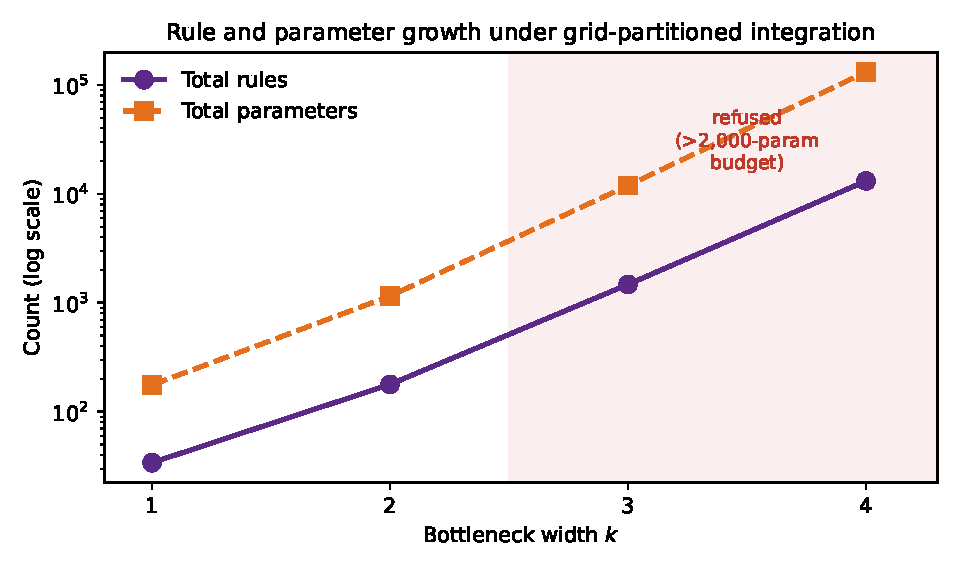
\includegraphics[width=0.75\linewidth]{fig_e5_rule_growth.pdf}
\caption{Rule and parameter growth with bottleneck width $k$ under grid partition of the integration
tier. The shaded region ($k\ge3$) exceeds the parameter budget the present inventory supports and was
refused rather than attempted.}\label{fig:e5-rule-growth}
\end{figure}

At $k{=}1$ the sweep uses exactly A-09's training scheme: the alternating closed-form least squares
for both lower panels, the intercept refit after the monotone projection, and the same hard clamp on
$v,e$ that HANFIS's own forward pass applies. It is implemented separately in
\texttt{hanfis\_bottleneck.py} under a multi-head representation that generalises cleanly to $k>1$. A
per-row comparison against the $k{=}1$ predictions underlying Table~\ref{tab:e4-results} confirms this
reproduction directly: Pearson $r=0.9984$ on point predictions, and
identical fold assignment for all 981 held-out rows. An earlier version of this sweep used a simpler
training scheme (the Integration-only closed form rather than the alternating scheme) and omitted the
intercept refit after the monotone projection; both have since been corrected, and the numbers below
supersede that earlier, confounded comparison.

\begin{table}[h]
\caption{E5 bottleneck-width sweep: pooled RMSE and skill against persistence, 95\% confidence intervals
from 2{,}000 image-clustered bootstrap resamples (the same procedure as
Table~\ref{tab:e4-results}), 120-asset inventory.}\label{tab:e5-results}
\begin{tabular}{@{}lccc@{}}
\toprule
$k$ & Rules / Params & RMSE (pooled) & $\mathrm{SS}_{\mathrm{pers}}$ [95\% CI] \\
\midrule
1 & 34 / 176 & 0.587 & 0.169\ [$-0.330$,\ 0.343] \\
2 & 178 / 1152 & 0.820 & $-0.622$\ [$-2.259$,\ $-0.100$] \\
\botrule
\end{tabular}
\end{table}

\begin{figure}[h]
\centering
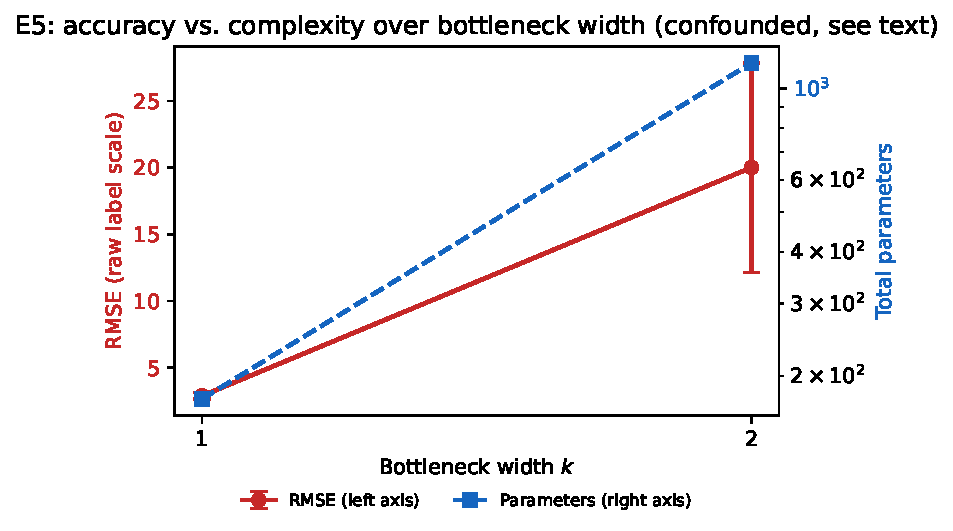
\includegraphics[width=0.75\linewidth]{fig_e5_bottleneck_curve.pdf}
\caption{E5: pooled skill against persistence for $k\in\{1,2\}$ with 95\% image-clustered bootstrap
confidence intervals. $k{=}1$'s interval now crosses zero; $k{=}2$'s is entirely
negative.}\label{fig:e5-bottleneck-curve}
\end{figure}

$k{=}1$ recovers skill broadly consistent with HANFIS's own H1b result (Table~\ref{tab:e4-results}: $\mathrm{SS}_{\mathrm{pers}}=0.015$, $[-0.607,0.246]$). Both confidence intervals cross zero and overlap substantially, as the per-row parity above predicts, though the point estimates ($0.169$ vs.\ $0.015$) agree less closely than on the smaller inventory. $k{=}2$'s interval now excludes zero entirely on the negative side. On the completed 120-asset inventory, widening the bottleneck is significantly worse than persistence. On the smaller inventory it had been unsupported by the evidence but not shown to be worse. The paired comparison on matched resampled images (the same resample is used for both arms, so sampling noise is shared) gives $\mathrm{SS}_{\mathrm{pers}}(k{=}1)-\mathrm{SS}_{\mathrm{pers}}(k{=}2)=0.791$, 95\% CI $[0.354,2.037]$, which excludes zero (100\% of resamples favour $k{=}1$). $k{=}1$ is also pooled-RMSE-better on all five folds (two-sided sign test $p=0.0625$, the floor attainable with five folds). This is the same margin of evidence as on the smaller inventory, even though each arm's marginal significance against persistence flipped in opposite directions.

This is the strongest statement the present inventory supports. It is a mechanism claim, not a claim that wider bottlenecks are intrinsically worse: every $k{=}2$ fold falls under ten observations per parameter (range 0.3--2.9), the same ten-per-parameter threshold applied elsewhere in this study (Section~\ref{subsec:target-definition}), while $k{=}1$ clears it in three of five folds. A secondary diagnostic separates part of this gap from pure data scarcity. Disabling the hard clamp on $v,e$ (an ablation, not the model HANFIS reports) costs $k{=}1$ 0.161 of skill but costs $k{=}2$ 0.813. Both were re-run on the completed 120-asset inventory; the costs were 0.019 and 0.394 respectively on the 27-image pilot. This is consistent with $v,e$ being estimated less reliably from the same training rows once six times as many consequent parameters compete for them, so that excursions outside $[0,1]$ are both more frequent and more consequential once clamped. Separating an intrinsic cost of wider bottlenecks from this data-scale effect requires an inventory substantially larger than the 120 assets collected here, which is left for future work. The architecture's own combinatorial growth in $k$ (Figure~\ref{fig:e5-rule-growth}) means that this separation gets harder, not easier, as $k$ increases.

\subsection{Ablation and robustness analysis}\label{subssec4.5}
Table~S2 of Additional file~1 reports the membership-family$\times$monotonicity ablation (E1) on two synthetic scenarios (S1 smooth, S2 with a hard threshold; five seeds per cell). The monotonicity constraint costs little on the smooth scenario but is expensive on the threshold scenario for the Gaussian family (RMSE $0.117\to6.067$), because softplus-constrained slopes cannot represent a local reversal; the connected Ruspini family degrades far less ($0.646\to2.126$). Amendment A-10 therefore keeps the Gaussian family with monotonicity active as the frozen default and treats Ruspini as a documented, cheaper fallback. An end-to-end pure-Adam variant without the closed-form anchor (Section~\ref{subsec:hanfis-architecture}) diverged on a subset of seeds, confirming that the hybrid scheme is necessary.

\emph{Sensitivity to the EPSS model change.} The EPSS scoring model changed version on 2026-06-15 (\texttt{v2025.03.14} to \texttt{v2026.06.15}). In a post hoc sensitivity analysis, the confirmatory pipeline was re-run on the 4{,}560 asset-weeks whose labels all pre-date the change (720 held-out rows; Table~S3 of Additional file~1). H1a, H1c and H2 remain confirmed, and H1b remains unconfirmed, with a much wider interval.

\emph{Where HANFIS and persistence differ.} The pooled skill against persistence ($0.015$) hides two regimes (exploratory, post hoc, outside the Holm-corrected family). For the four weeks in which the label is fully computed under the new EPSS model while the lagged label is still computed under the old one (2026-W24 to W27; 95 rows), skill against persistence is $+0.483$; on the remaining 985 rows it is $-0.420$. HANFIS is therefore reactive rather than predictive: better than persistence when the label moves, worse when it does not. Two further observations qualify H2. The first held-out fold, trained on 2.2 observations per parameter, contributes $91\%$ of the pooled gap to the matched model; without it the skill against FlatANFISMatched is $0.183$ and against the full flat model $0.084$. The fold-by-fold and week-by-week values are in Supplementary note S2 of Additional file~1.

\subsection{Explanation fidelity (E6)}\label{sec:e6}
We tested whether the rule-level explanation that HANFIS exposes is faithful to its inference, using the 25 saved models (five folds $\times$ five seeds), which reproduce the confirmatory predictions exactly. The version-control freeze preceded the commit that contained the protocol text, so the protocol is not frozen in the strict sense and the run is reported as a documented deviation; Table~S4 of Additional file~1 lists the outcome. The rule-attribution check failed its criterion: removing the three rules ranked highest by attribution changed the output 4.1 times more than removing three random rules, but it exceeded the median random removal in only 83.5\% of non-degenerate rows (criterion: 90\%). Of the 575 positive-control pairs, 552 increased strictly. We therefore do not claim validated rule-level explanations: the rule trace matches the inference exactly and the direction of the response is verified, but the attribution of the output to individual rules is faithful on average rather than uniformly. The degenerate rows, the post hoc fold breakdown and the paired-week contrast are in Supplementary note S3 of Additional file~1.

\subsection{Attribution and monotonicity checks (E8)}\label{subsec:e8}
We computed exact interventional Shapley values~\cite{shapley1953value} for the seven inputs of the 25 saved models (5{,}400 model--row pairs; a background of 60 random labelled rows, excluding P0 and P0-IF and identical for all models; the efficiency property holds to $2\times10^{-14}$). Exploitability ($x_2$) and the KEV indicator ($x_7$), both ingredients of the label, carry 78.9\% of the mean absolute attribution; the three environment inputs ($x_4$--$x_6$) carry 3.3\% (Table~\ref{tab:e8}). The ranking is stable across models (Kendall $W=0.79$; $x_2$ is the top input in 21 of 25 models), and in the 20\% of rows with the highest label $x_7$ alone carries 63.0\%. This quantifies the overlap between label and inputs discussed in Section~\ref{sec5}: the model largely forecasts exploitability signals it can already see, and the label contains no environment component by construction.

\begin{table}[ht]
\caption{Exact Shapley attribution and within-row monotonicity checks for the five-seed ensemble (E8; descriptive and post hoc). ``Falls'' is the share of steps, over the range observed in the data, in which the score drops by more than 0.05 points when one input is raised and the others are held fixed. Share: mean absolute attribution; Max drop and Range: largest fall and mean end-to-end change of the score in points.}\label{tab:e8}
\begin{tabular}{@{}p{0.36\linewidth}rrrr@{}}
\hline
Input & Share (\%) & Falls (\%) & Max drop & Range\\
\hline
$x_1$ CVSS & 10.9 & 1.7 & 2.46 & 1.99\\
$x_2$ Exploitability & 46.4 & 1.2 & 0.21 & 6.53\\
$x_3$ Patch Risk & 6.8 & 24.8 & 2.28 & 1.11\\
$x_4$ MFA Risk & 1.1 & 29.1 & 0.46 & 0.09\\
$x_5$ Kubernetes Exposure & 1.3 & 34.8 & 0.60 & 0.14\\
$x_6$ Asset Criticality & 0.9 & 10.5 & 0.40 & 0.13\\
$x_7$ Threat Intelligence (KEV) & 32.5 & 1.2 & 0.33 & 6.45\\
\hline
\end{tabular}
\end{table}

Non-negative rule slopes do not guarantee a monotone score, because rule weights are normalised and intercepts are free. We therefore varied one input at a time over 11 points spanning the observed range (observed values for discrete inputs, quantiles from 1\% to 99\% otherwise) for the five-seed ensemble that is reported in Section~\ref{sec4}. For the dominant drivers the share of falling steps is small ($x_1$ 1.7\%, $x_2$ 1.2\%, $x_7$ 1.2\%), whereas for patch risk and the environment inputs it is 10--35\%, although the environment inputs move the score by less than 0.15 points on average (Table~\ref{tab:e8}). Individual seeds are less well behaved than the ensemble: the largest single drop (11.6 points, CVSS) occurs in one seed on two assets in the last held-out block, after the EPSS model change. We therefore present monotonicity as an empirical property of the dominant inputs, not as a guarantee of the architecture.

\subsection{Label-ingredient ablation and information-minimal baselines (E9--E11)}\label{subsec:e9}
Both analyses were designed after the attribution results of Section~\ref{subsec:e8} and are therefore post hoc. In E9 we retrained HANFIS with $x_2$ and $x_7$ replaced by the constant zero in training and test data, on the folds, seeds, embargo, validation split and hyperparameters of the confirmatory run, which we verified to reproduce the same 1{,}080 held-out rows. Skill scores are $\mathrm{SS}=1-\mathrm{MSE}_{\mathrm{model}}/\mathrm{MSE}_{\mathrm{reference}}$ with 95\% bootstrap intervals clustered by image (2{,}000 resamples). Without the two label ingredients the five-seed ensemble has a mean squared error of 14.23, against 0.41 with them and 12.54 for a single CVSS score. Its skill over CVSS is $-0.135$ (interval $[-0.336,\,0.046]$) and over a ridge model on the remaining five inputs $-0.070$ ($[-0.250,\,0.096]$). That ridge model is itself no better than CVSS ($-0.061$, $[-0.130,\,0.006]$). On this inventory the remaining inputs therefore carry no demonstrable information beyond CVSS, and essentially all of the model's skill comes from the two inputs that are also ingredients of the label.

In E10 we compared the confirmatory HANFIS predictions with the simplest functions of those inputs, trained on the same rows: a plug-in $100\,x_2$, ridge regression on $(x_2,x_7)$, and gradient boosting on $(x_2,x_7)$, on all seven inputs, and on the seven inputs plus the four-week lag of the label (Table~\ref{tab:e9}). Within this group, HANFIS has a lower error than every alternative with an interval excluding zero, except gradient boosting restricted to $x_2$ and $x_7$ (skill $0.606$, interval $[-0.079,\,0.847]$). Adding the other inputs makes gradient boosting worse, not better, and models that receive the lagged label as a feature do much worse than the lag itself, which we attribute, without having tested it, to distribution shift between training and test periods. Taken alone, these comparisons would suggest that HANFIS is a compact estimator of exposure from $x_2$ and $x_7$ that matches persistence without access to past labels; the next comparison qualifies this.

In E11 we asked whether a small formula suffices. Because the label is the window mean of a maximum over $\max(\mathrm{EPSS},\mathbb{1}[\mathrm{KEV}])\,\rho$, we fitted $\hat y=a+b\,\max(x_2,\,c\,x_7)$ on the training rows of each fold, choosing $c$ on a grid and $a,b$ by least squares, together with a ridge model with the $x_2x_7$ interaction and monotone gradient boosting on $(x_2,x_7)$. The grid selected $c=0.10$ in all five folds, with $b$ between 99.2 and 100.0 and $a<0.07$, that is, almost exactly $100\max(x_2,\,0.1\,x_7)$. This formula has a lower pooled error (0.27) than HANFIS (0.41) and than persistence (0.42). HANFIS is worse than the formula, with a skill of $-0.534$ (interval $[-1.438,\,-0.208]$), and worse than the interaction ridge ($-0.529$), while it is not distinguishable from monotone boosting ($0.538$, $[-0.005,\,0.802]$). We had expected parity or an advantage for HANFIS; the observed disadvantage means that on this target the 176-parameter model adds no accuracy to what a four-parameter formula of current EPSS and KEV signals already provides. The gains over CVSS, linear models and a flat ANFIS reported in the confirmatory comparisons therefore show that the task is nearly determined by those two signals, not that the hierarchical structure helps.

\begin{table}[ht]
\caption{Label-ingredient ablation (E9), information-minimal baselines (E10) and formula baselines (E11), 1{,}080 held-out rows. Skill score with 95\% image-clustered bootstrap interval; MSE of the model and of the reference.}\label{tab:e9}
\small
\begin{tabular}{@{}p{0.38\linewidth}rrr@{}}
\hline
Comparison & Skill & 95\% interval & MSE\\
\hline
\multicolumn{4}{@{}l}{\emph{E9: HANFIS retrained without $x_2$ and $x_7$}}\\
vs.\ CVSS only & $-0.135$ & $[-0.336,\,0.046]$ & 14.23 / 12.54\\
vs.\ ridge, remaining five inputs & $-0.070$ & $[-0.250,\,0.096]$ & 14.23 / 13.30\\
vs.\ HANFIS with all inputs & $-33.8$ & $[-56.5,\,-22.5]$ & 14.23 / 0.41\\
Ridge, five inputs, vs.\ CVSS only & $-0.061$ & $[-0.130,\,0.006]$ & 13.30 / 12.54\\
\multicolumn{4}{@{}l}{\emph{E10: HANFIS with all inputs vs.}}\\
Plug-in $100\,x_2$ & $0.859$ & $[0.672,\,0.931]$ & 0.41 / 2.89\\
Ridge on $(x_2,x_7)$ & $0.693$ & $[0.518,\,0.817]$ & 0.41 / 1.33\\
Ridge on lag-4 label, $x_2$, $x_7$ & $0.635$ & $[0.399,\,0.781]$ & 0.41 / 1.12\\
Boosting on $(x_2,x_7)$ & $0.606$ & $[-0.079,\,0.847]$ & 0.41 / 1.04\\
Boosting on seven inputs & $0.659$ & $[0.133,\,0.860]$ & 0.41 / 1.20\\
Boosting on lag-4 label and inputs & $0.653$ & $[0.104,\,0.858]$ & 0.41 / 1.18\\
Persistence (lag-4 label) & $0.015$ & $[-0.620,\,0.243]$ & 0.41 / 0.42\\
\multicolumn{4}{@{}l}{\emph{E11: HANFIS with all inputs vs.}}\\
Max-form formula $a+b\max(x_2,c\,x_7)$ & $-0.534$ & $[-1.438,\,-0.208]$ & 0.41 / 0.27\\
Ridge on $x_2$, $x_7$, $x_2x_7$ & $-0.529$ & $[-1.415,\,-0.206]$ & 0.41 / 0.27\\
Monotone boosting on $(x_2,x_7)$ & $0.538$ & $[-0.005,\,0.802]$ & 0.41 / 0.88\\
\hline
\end{tabular}
\end{table}

\subsection{Horizon sweep and feature impact by horizon (E14)}\label{subsec:e14}
All preceding analyses use the four-week label window of the confirmatory protocol. To check whether the conclusions depend on that horizon, we rebuilt the dataset with label windows of 58 and 86 days (eight and twelve weekly snapshots after $t$). To avoid leakage we set the persistence lag and the embargo to the window length (8 and 12 weeks; 58 and 86 days). We then repeated the out-of-fold comparison of HANFIS, the max-form formula and persistence with the same folds, seeds and hyperparameters. Longer windows leave fewer labelled weeks (the last labelled week is 2026-07-27 and 2026-06-29), so the out-of-fold samples shrink to 889 and 697 rows, and mean squared errors at different horizons are not comparable because the labels average different numbers of snapshots; only skill scores are compared. This analysis is post hoc.

The formula's advantage over persistence is stable (skill $0.36$, $0.49$ and $0.44$ at four, eight and twelve weeks), whereas the gap between HANFIS and the formula closes: $-0.534$ (interval $[-1.438,\,-0.208]$) at four weeks, $-0.048$ ($[-0.205,\,0.032]$) at eight and $0.039$ ($[-0.031,\,0.110]$) at twelve. HANFIS beats persistence from eight weeks on ($0.467$ and $0.462$, intervals above zero). Because the longer horizons only contain older weeks (the EPSS model changed on 2026-06-15), horizon and period are confounded. Restricting all three horizons to the 408 asset-weeks present in each, the pattern remains: the skill of HANFIS against the formula changes by $+0.862$ ($[+0.309,\,+2.973]$) between four and twelve weeks, while the skill of the formula against persistence does not change ($-0.016$, $[-0.096,\,+0.141]$).

Removing exploitability and the KEV indicator again removes all skill at eight and twelve weeks (skill against CVSS alone $-0.099$ and $-0.179$, intervals including or touching zero; against HANFIS with all inputs $-24.0$ and $-14.6$). A ridge model on the remaining five inputs is not better than CVSS alone ($-0.069$ and $-0.071$). The relative gain of HANFIS at longer horizons does not come from the other inputs; Section~\ref{subsec:e16} shows that it is largely due to weeks around the EPSS model change and that on unaffected rows HANFIS remains behind the formula. The evidence is suggestive, not conclusive: at twelve weeks HANFIS and the formula are not distinguishable, cross-fitted blends of the two do not improve on either alone, and the forward evaluation planned for the confirmatory protocol covers only the four-week horizon.

\begin{table}[ht]
\caption{Horizon sweep (E14, post hoc). Skill score with 95\% image-clustered bootstrap interval. Panel A: all out-of-fold rows; B: the 408 asset-weeks present at all three horizons; C: HANFIS retrained without $x_2$ and $x_7$ against CVSS only.}\label{tab:e14}
\small
\begin{tabular}{@{}p{0.47\linewidth}rrr@{}}
\hline
Comparison & Skill & 95\% interval & Rows\\
\hline
\multicolumn{4}{@{}l}{\emph{A. All out-of-fold rows}}\\
4 weeks: formula vs.\ persistence & $0.357$ & $[0.279,\,0.407]$ & 1080\\
4 weeks: HANFIS vs.\ persistence & $0.015$ & $[-0.620,\,0.243]$ & 1080\\
4 weeks: HANFIS vs.\ formula & $-0.534$ & $[-1.438,\,-0.208]$ & 1080\\
8 weeks: formula vs.\ persistence & $0.492$ & $[0.269,\,0.696]$ & 889\\
8 weeks: HANFIS vs.\ persistence & $0.467$ & $[0.236,\,0.651]$ & 889\\
8 weeks: HANFIS vs.\ formula & $-0.048$ & $[-0.205,\,0.032]$ & 889\\
12 weeks: formula vs.\ persistence & $0.440$ & $[0.245,\,0.597]$ & 697\\
12 weeks: HANFIS vs.\ persistence & $0.462$ & $[0.277,\,0.610]$ & 697\\
12 weeks: HANFIS vs.\ formula & $0.039$ & $[-0.031,\,0.110]$ & 697\\
\multicolumn{4}{@{}l}{\emph{B. Same 408 asset-weeks at every horizon}}\\
4 weeks: HANFIS vs.\ formula & $-0.812$ & $[-2.952,\,-0.264]$ & 408\\
8 weeks: HANFIS vs.\ formula & $-0.045$ & $[-0.218,\,0.038]$ & 408\\
12 weeks: HANFIS vs.\ formula & $0.050$ & $[-0.060,\,0.158]$ & 408\\
Change 12 minus 4 weeks: HANFIS vs.\ formula & $0.862$ & $[0.309,\,2.973]$ & 408\\
Change 12 minus 4 weeks: formula vs.\ persistence & $-0.016$ & $[-0.096,\,0.141]$ & 408\\
\multicolumn{4}{@{}l}{\emph{C. HANFIS without $x_2$, $x_7$ vs.\ CVSS only}}\\
4 weeks & $-0.135$ & $[-0.336,\,0.046]$ & 1080\\
8 weeks & $-0.099$ & $[-0.289,\,0.069]$ & 889\\
12 weeks & $-0.179$ & $[-0.406,\,0.007]$ & 697\\
\hline
\end{tabular}
\end{table}

\subsection{Prioritisation utility (E15)}\label{subsec:e15}
Risk scores are used to rank assets, so we also compared the predictors on ranking within each week (post hoc; out-of-fold predictions at three horizons; weekly Spearman correlation and precision at the top 20\%; Tables~S5 and~S6 of Additional file~1). All predictors rank assets almost identically. At four weeks the weekly Spearman correlation is $0.99$ for the formula and for persistence and $0.97$ for HANFIS, and the precision at the top 20\% is $0.97$ for all three, so the lower squared error of the formula does not translate into a practical gain in prioritisation. At longer horizons the differences stay small (Supplementary note S4 of Additional file~1), and with eighteen paired comparisons and no correction for multiplicity the intervals are descriptive.

\subsection{Error anatomy and the EPSS model change (E16--E19)}\label{subsec:e16}
The preceding sections compare pooled errors. To see where the differences come from, we analysed the four-week out-of-fold predictions by stratum, by time block and by distance to the change of the EPSS model on 2026-06-15 (post hoc, with a bootstrap clustered by image).

\emph{Reactivity.} The advantage of the formula over persistence is concentrated in rows in which an input changed during the previous four weeks (628 of 1{,}080 rows): its skill is $0.400$ (interval $0.308$ to $0.487$) there and $0.002$ ($-0.069$ to $0.037$) where nothing changed (Table~S7 of Additional file~1). HANFIS has skill $0.125$ in changed rows and $-0.900$ ($-4.171$ to $-0.206$) in unchanged rows: it adds noise where persistence is already adequate. A gate that returns persistence in unchanged rows removes this deficit but leaves HANFIS no better than persistence ($0.111$, $-0.367$ to $0.292$) and worse than the formula ($-0.383$, $-0.998$ to $-0.131$).

\emph{The model change.} The largest errors are small shifts of the score in the weeks 2026-W21 to W24, whose four-week label windows straddle the EPSS model change: $x_2$ is computed with the old model while the label, and the label of the persistence forecast, use the new one. Rows within the label window of the change (190 of 1{,}080 at four weeks) hold 77\% of the squared error of persistence and of the formula and 49\% of that of HANFIS. On the remaining rows (Table~\ref{tab:e19}) the formula keeps its point estimate of skill against persistence ($0.348$ against $0.357$) but the interval now includes zero ($-0.060$ to $0.422$); HANFIS is significantly worse than persistence ($-1.228$) and than the formula ($-2.418$). The forward evaluation (Section~\ref{subsec:e7-results}) is free of this change. At eight and twelve weeks the gap between HANFIS and the formula narrows (Section~\ref{subsec:e14}), but on rows unaffected by the change HANFIS stays behind the formula ($-0.324$ and $-0.362$, intervals including zero): the horizon sweep shows a shrinking deficit, not parity. The concentration of error, the leave-one-block-out estimates and the common-weeks analysis are in Supplementary note S5 of Additional file~1.

\begin{table}[ht]
\caption{Skill on all out-of-fold rows and on rows unaffected by the EPSS model change (E19, post hoc), with 95\% image-bootstrap intervals from a separate run (they differ slightly from Table~\ref{tab:e14}). Unaffected rows: 890 of 1{,}080 (four weeks), 536 of 889 (eight) and 342 of 697 (twelve).}\label{tab:e19}
\footnotesize
\setlength{\tabcolsep}{3pt}
\begin{tabular}{@{}p{0.32\linewidth}p{0.29\linewidth}p{0.29\linewidth}@{}}
\hline
Comparison & All rows & Unaffected rows\\
\hline
4 w: formula vs.\ persistence & $0.357$ $[0.279,\,0.407]$ & $0.348$ $[-0.060,\,0.422]$\\
4 w: HANFIS vs.\ persistence & $0.015$ $[-0.627,\,0.252]$ & $-1.228$ $[-12.804,\,-0.015]$\\
4 w: HANFIS vs.\ formula & $-0.534$ $[-1.383,\,-0.204]$ & $-2.418$ $[-13.204,\,-0.709]$\\
8 w: formula vs.\ persistence & $0.492$ $[0.269,\,0.696]$ & $0.623$ $[-0.009,\,0.699]$\\
8 w: HANFIS vs.\ persistence & $0.467$ $[0.241,\,0.670]$ & $0.501$ $[-1.631,\,0.702]$\\
8 w: HANFIS vs.\ formula & $-0.048$ $[-0.200,\,0.036]$ & $-0.324$ $[-2.153,\,0.052]$\\
12 w: formula vs.\ persistence & $0.440$ $[0.245,\,0.597]$ & $0.824$ $[0.270,\,0.913]$\\
12 w: HANFIS vs.\ persistence & $0.462$ $[0.269,\,0.614]$ & $0.761$ $[-0.220,\,0.888]$\\
12 w: HANFIS vs.\ formula & $0.039$ $[-0.034,\,0.106]$ & $-0.362$ $[-1.342,\,0.018]$\\
\hline
\end{tabular}
\end{table}

\subsection{Calibration (E21)}\label{subsec:e21}
We checked calibration after the registration of the forward evaluation had become public (post hoc, descriptive, no training); Table~S8 of Additional file~1 gives the details. All three predictors lie close to the identity line. Persistence runs low on all rows (mean error $-0.097$, interval $-0.196$ to $-0.013$), almost entirely because of the weeks around the EPSS model change (on unaffected rows $-0.015$, $-0.079$ to $0.025$). HANFIS departs most: its slope is $1.025$ ($1.008$ to $1.044$) on all rows and $1.031$ ($1.014$ to $1.053$) on unaffected rows, where its intercept is $-0.193$ ($-0.300$ to $-0.085$). These departures are small next to the label scale, and a bootstrap clustered by week (E22) gives narrower, not wider, intervals for them. We read the miscalibration of HANFIS as small but consistent in slope and intercept where the model change does not interfere, and as descriptive.

A linear recalibration (E23, post hoc) does not close the gap between HANFIS and the formula: on all rows the skill of HANFIS against the formula is $-0.534$ ($-1.383$ to $-0.204$) before and $-0.535$ ($-1.287$ to $-0.232$) after cross-fitted recalibration, so the deficit is not explained by a linear miscalibration. Stacking (E24, post hoc) finds no information in HANFIS that a straight line can use: the skill of the combination against the recalibrated formula is $-0.001$ ($-0.006$ to $0.004$) on all rows. The full descriptions and all intervals are in Supplementary note S6 of Additional file~1.

\subsection{Prospective evaluation (E7): forward results}\label{subsec:e7-results}
The design of Section~\ref{subsec:e7} was executed once on 2026-11-02, and no stage was repeated. The evaluation covers 6 forward weeks (2026-08-31 to 2026-10-05) and 720 asset-weeks from 120 images (119 image groups). No row was dropped under the pre-registered insufficient-evidence rule, so every asset stayed in the analysis, including \texttt{cockroachdb}. The EPSS model version stayed at v2026.06.15 throughout.

Table~\ref{tab:e7-results} lists the registered decisions. In weeks without an EPSS model change, HANFIS was not better than persistence: the skill score was $-3.757$ (95\% CI $-9.177$ to $-1.594$), and the upper bound lies below the margin of $0.05$ (P7a supported). The fixed blend was worse than persistence (SS $-0.807$, 95\% CI $-2.507$ to $-0.160$). The max-form formula beat persistence (SS $0.340$, 95\% CI $0.060$ to $0.628$; MSE $0.261$ against $0.396$; one-sided $p=0.0005$, Holm threshold $0.0125$). P7e is confirmed. HANFIS was not better than the formula (SS $-6.208$, 95\% CI $-13.677$ to $-3.188$; MSE $1.884$ for HANFIS against $0.261$ for the formula). The upper bound lies below $0.05$, so P7f is supported. The mean weekly Spearman correlation between predicted and realised change was $0.066$ (lower 95\% bound $-0.074$); the lower bound does not exceed zero, so P7d is not demonstrated. A bootstrap clustered by week (6 weeks) gives the same decision for P7e and P7f (SS $0.340$, 95\% CI $0.100$ to $0.758$ for P7e). The reported $p$ values equal $1/2001$, the smallest value that a bootstrap of 2{,}000 resamples can give.

\begin{table}[h]
\caption{E7 forward results: skill score (pooled mean squared error, bootstrap clustered by image, 2{,}000 resamples) with 95\% CI. P7a and P7b form one Holm family, P7e and P7f another; P7e and P7f are post hoc in origin.}\label{tab:e7-results}
\begin{tabular}{@{}llccl@{}}
\toprule
Hypothesis & Comparison & SS & 95\% CI & Decision \\
\midrule
P7a & HANFIS against persistence & $-3.757$ & [$-$9.177, $-$1.594] & Supported \\
P7b & Blend against persistence & $-0.807$ & [$-$2.507, $-$0.160] & Worse \\
P7e & Formula against persistence & 0.340 & [0.060, 0.628] & Confirmed \\
P7f & HANFIS against formula & $-6.208$ & [$-$13.677, $-$3.188] & Supported \\
\botrule
\end{tabular}
\end{table}

Against the out-of-fold results of Section~\ref{subsec:e9}, where the MSE was 0.27 for the formula, 0.42 for persistence and 0.41 for HANFIS, the forward MSE of the formula (0.261) and of persistence (0.396) stayed close, while that of HANFIS rose to 1.884.

P7e and P7f have a post hoc origin: they were added to the protocol before the freeze but derive from analyses of earlier data (E11 to E14). The protocol is tagged \texttt{e7-prereg-2026-10-12} (commit \texttt{dbed812}) and registered on the Open Science Framework (\texttt{https://osf.io/ahcvs/}; DOI \texttt{10.17605/OSF.IO/AHCVS}); the forward outputs are tagged \texttt{e7-results-2026-11-02}, and a Zenodo version DOI will be added. This is one forward window of six weeks and 120 images with shared weekly shocks, so the result does not extend to other EPSS model versions or to other image sets. Analyses after the freeze (E14c and E15 to E24) are post hoc and descriptive; none of them changes a registered decision.

\section{Discussion}\label{sec5}

Three findings from the completed experiments (E1, E3, and the observability-overhead runs) shape how the confirmatory comparison in Section~\ref{subssec4.3} should be read. First, the label is dominated by its own recent history. A 4-week persistence forecast reduces mean squared error relative to climatology by 97\% on the 120-asset inventory (Table~\ref{tab:e3-baselines}; 96\% on the earlier pilot), so any claim that HANFIS ``predicts risk'' is a claim about improving on a strong autoregressive baseline, not about beating an uninformative one. This is why H1 was reframed against persistence rather than against Fuzzyfortify or CVSS alone (Section~\ref{sec1}). Second, a single CVSS score has limited explanatory power for the realised 30-day exploitability exposure ($\mathrm{SS}_{\mathrm{clim}}=0.222$ on the 120-asset inventory, against about 0 on the earlier pilot). Severity and realised exploitation are different quantities, and conflating them is a plausible source of alert fatigue in practice; this is consistent with the research gap that C3 claims to address. Third, the E1 ablation shows that a monotonicity constraint intended to keep the model auditable (higher risk factors must not lower the score) has a real, family-dependent accuracy cost on data containing thresholds. Choosing Gaussian membership functions with monotonicity active therefore trades some accuracy for a response that, for the dominant risk factors, rarely falls as they rise (Section~\ref{subsec:e8}); it was a deliberate choice.

The post hoc analyses of Sections~\ref{subsec:e8} and~\ref{subsec:e9} limit how far these findings generalise. Exact Shapley attribution places 78.9\% of the model's attribution on exploitability and the KEV indicator, which are ingredients of the realised label, and only 3.3\% on the three environmental inputs. Without those two inputs the model shows no demonstrable skill over a single CVSS score, and it is not demonstrably better than gradient boosting restricted to them. What the data support is therefore narrower. A 34-rule hierarchical model estimates near-term exploitability exposure from current EPSS and KEV signals about as accurately as a persistence forecast that needs past labels (the two are not distinguishable), and more accurately than generic linear and boosted models. It is not more accurate than a four-parameter formula of the same two signals (Section~\ref{subsec:e9}); this formula, together with the interaction ridge, has the lowest error of all predictors we compared at the four-week horizon. At eight and twelve weeks the gap to the formula narrows, but only through weeks around the EPSS model change (Sections~\ref{subsec:e14} and~\ref{subsec:e16}). The ranking of assets by predicted risk is almost the same for all predictors at four weeks (Section~\ref{subsec:e15}). The data do not support the claim that the vulnerability--environment decomposition, or the environmental inputs, improve prediction. Because the target is built from EPSS, KEV and reachability alone and does not depend on the three environmental inputs, this inventory is not designed to show a benefit of those inputs even if one exists; testing that benefit requires an outcome that depends on the environment, such as incident or impact data. Forward weeks confirm the earlier finding: a max-form formula in the exploitability and threat-intelligence inputs matches or beats the trained model, and HANFIS adds structure and a readable rule base, not accuracy (Section~\ref{subsec:e7-results}). In those weeks HANFIS was not better than persistence (P7a) and its blend with persistence was worse than persistence alone (P7b). We did not test why the trained model transferred worse than the formula.

The instrumentation-overhead results (Section~\ref{subsec4.1}) support a second, narrower claim: Kubernetes observability telemetry can be treated as a fixed resource cost rather than folded into the risk model as a confound. Node-level CPU increases by 99.4~mCPU under monitoring, while the monitoring namespace itself accounts for only 39.8~mCPU, so pod-level accounting alone understates the platform cost by a factor of about 2.5. Workload latency nonetheless shows no detectable change (95\% confidence intervals within $\pm 0.27$~ms). The cost of observing the system is thus separated from any change in the system being observed, which is the premise behind the Kubernetes-exposure input of the environmental subsystem. Whether that input improves prediction is a separate question, and on the present inventory the environmental inputs add no demonstrable predictive information (Section~\ref{subsec:e9}).

\subsection{Limitations}
Two limits of construct validity come first. First, the label and two of the inputs share ingredients: $x_2$ (EPSS $\times\,\rho$) and $x_7$ (the KEV indicator) are the values at $t$ of quantities that the label aggregates over $t{+}7,\dots,t{+}28$, and runtime reachability $\rho$ enters both. The task is therefore to forecast the near future of exploitability signals that the model can already see, not to predict independent compromise outcomes, for which no ground truth exists here. The persistence baseline, built in the same way, is the relevant bar, and the comparison with a single CVSS score should be read in that light. The exact Shapley attribution (Section~\ref{subsec:e8}) and the ablation without these two inputs (Section~\ref{subsec:e9}) show how heavily the model's skill rests on them. Second, the dynamic character of the score comes from the time-varying EPSS and KEV feeds and from runtime reachability. Runtime telemetry (CPU, memory, latency) is used only to quantify observability overhead and is not a model input, so ``dynamic'' must not be read as telemetry-driven scoring. The rule-level attribution is faithful on average but not uniformly (Section~\ref{sec:e6}), and we do not claim validated explanations.

\label{subsec5.1}

All analyses labelled post hoc were designed after the confirmatory results and run on the same data; they are descriptive, carry no multiplicity correction, and none of them changes a registered decision.

The inventory consists of public container images and a small number of testbed assets built from a public base image, and the label reflects exploitation signals of public vulnerabilities (EPSS, KEV), not incidents in a specific organisation; generalisation to other workloads or to incident-based outcomes is untested.

Three data-related caveats are detailed in Supplementary note S7 of Additional file~1. On the 120-asset inventory (6{,}357 labelled rows; Table~\ref{tab:e3-baselines}), a linear ridge model over all seven inputs underperforms persistence on every one of the five grouped-temporal folds ($\mathrm{SS}_{\mathrm{pers}}=-2.293$ pooled, raw scale), and we did not test why. The EPSS scoring model changed version (\texttt{v2025.03.14} to \texttt{v2026.06.15}) inside the sealed 57-week window, a threat to label comparability; a post hoc re-analysis restricted to weeks whose labels all pre-date the change leaves the confirmatory conclusions unchanged (Section~\ref{subssec4.5}). The data-sufficiency gate (at least ten observations per parameter) is met by the pooled sample ($6{,}357$ labelled rows against 176 parameters) but not by the two earliest held-out folds ($2.2$ and $7.1$ observations per parameter), which are also those in which HANFIS is furthest behind persistence; H2's pooled margin is dominated by the first fold (Section~\ref{subssec4.5}).

CVEs lacking a Trivy-reported publication date are dated by their first appearance in a sealed EPSS snapshot (at most 7 days late), and a single CVE whose Trivy status lies outside the accepted set makes the whole asset-week unusable; this affected one of the 120 images for seven consecutive weeks from 2026-08-10, and such rows are removed. Labels whose four-week window straddles the EPSS model change of 2026-06-15 (and the persistence labels derived from them) mix two score definitions; these rows (18\% of the out-of-fold rows) hold 77\% of the squared error of persistence and of the formula, and the forward evaluation avoids them. The label aggregation rule, its numeric scale and the definition of Patch Risk were closed and pre-registered as amendment A-13 before the confirmatory comparison in Table~\ref{tab:e4-results} was run.

The testbed is a
single two-node WSL~2/Docker Desktop Kubernetes cluster; external validity to production multi-node
clusters and other CNI/storage stacks is untested. Ten paired observability runs, while showing large
and consistent effects, still provide limited power for null-hypothesis testing on the latency measure
specifically, which is why the reported confidence intervals rather than a significance threshold carry
the interpretive weight in Section~\ref{subsec4.1}.

\section{Conclusion and Future Work}\label{sec6}

This paper proposes HANFIS, a domain-informed hierarchical ANFIS. It reduces a 128-rule, 1{,}052-parameter flat Sugeno system over seven cloud-native risk inputs to 34 rules and 176 parameters (Section~\ref{subsec:hanfis-architecture}) by separating vulnerability and environmental reasoning into two first-tier panels before an integration tier combines them with dynamic threat intelligence. Under a protocol frozen and dated before training began (Table~\ref{tab:e4-results}), HANFIS confirms a substantial reduction in estimation error against a single CVSS score (H1a), a linear model over the same seven inputs (H1c), and a parameter-matched flat ANFIS initialised by subtractive clustering (H2). It is not distinguishable from a causal 4-week persistence forecast (H1b), which the study's own mandatory baselines (Section~\ref{subssec4.3}) show to be a far harder bar than static expert scoring. The pooled margin over the matched model is dominated by the first block, where training is thinnest, so it is read as suggestive of a structural advantage of the vulnerability/environmental/threat decomposition, not as evidence for one (Section~\ref{subssec4.5}).

Post hoc analyses qualify this further. The model's skill rests on exploitability and KEV (78.9\% of the exact Shapley attribution; without them it has no skill over CVSS), and a four-parameter formula of those two inputs has a lower error than HANFIS (Sections~\ref{subsec:e8} and~\ref{subsec:e9}). On this target HANFIS therefore provides a compact rule base with a documented response surface, not better accuracy than a simple formula at the four-week horizon. The pre-registered forward evaluation (Section~\ref{subsec:e7-results}) points the same way: the accuracy of HANFIS on this task is bounded by a simple formula; its value lies in structure and interpretability. At eight and twelve weeks the gap narrows but does not close on rows unaffected by the EPSS model change, and the other inputs do not contribute (Sections~\ref{subsec:e14} and~\ref{subsec:e16}). Whether environmental context improves forecasts remains open. Two further contributions are established: the sealed, hash-verified real-world data pipeline (120 assets and 6{,}357 labelled asset-weeks, Section~\ref{subsec:target-definition}) and a completed ablation showing that the monotonicity constraint has a real, membership-family-dependent accuracy cost, met in practice only for the dominant drivers (Sections~\ref{subssec4.5} and~\ref{subsec:e8}).

H1b against persistence remains unconfirmed, and the forward weeks did not support it either (P7a). The bottleneck-width sweep (Section~\ref{subssec4.4}) found that widening the scalar inter-tier bottleneck from $k{=}1$ to $k{=}2$ does not close the gap to persistence; the wider model is significantly worse than persistence. Re-scanning every image with a single frozen vulnerability database, so that no image's CVE surface differs merely because it was scanned on a different day, was done once for the forward evaluation (Section~\ref{subsec:e7-results}); the earlier 57-week window still rests on scans from different days. The policy-translation layer (not a contribution of this paper) and edge deployment (originally hypothesis H5, now future work because the present testbed runs HANFIS cluster-side rather than on its edge node) remain designed but unevaluated. Both are left for a subsequent study.

\backmatter

\section*{List of abbreviations}

\begin{description}
\item[AI] Artificial intelligence
\item[ANFIS] Adaptive neuro-fuzzy inference system
\item[ANN] Artificial neural network
\item[CI] Confidence interval
\item[CISA] Cybersecurity and Infrastructure Security Agency
\item[CPU] Central processing unit
\item[CVE] Common Vulnerabilities and Exposures
\item[CVSS] Common Vulnerability Scoring System
\item[DOI] Digital Object Identifier
\item[EPSS] Exploit Prediction Scoring System
\item[FIS] Fuzzy inference system
\item[HANFIS] Hierarchical adaptive neuro-fuzzy inference system
\item[HTTP] Hypertext Transfer Protocol
\item[KEV] Known Exploited Vulnerabilities
\item[LPPM] Institute for Research and Community Service
\item[MFA] Multi-factor authentication
\item[MSE] Mean squared error
\item[OSF] Open Science Framework
\item[RMSE] Root mean squared error
\item[SHA] Secure Hash Algorithm
\item[SS] Skill score
\item[WSL] Windows Subsystem for Linux
\end{description}


\section*{Declarations}

\begin{itemize}
\item \textbf{Funding.} This work is supported by the Penelitian Kepakaran research grant, Institute for Research and Community Service (LPPM), Universitas Andalas, Indonesia. The funder had no role in the design of the study, in the collection, analysis or interpretation of data, or in writing the manuscript.
\item \textbf{Competing interests.} The authors declare no competing interests.
\item \textbf{Ethics approval and consent to participate.} Not applicable: this study involves no human participants, human data, or animal subjects. All measurements were collected from an isolated Kubernetes research testbed operated by the authors.
\item \textbf{Consent for publication.} Not applicable.
\item \textbf{Availability of data and materials.} The sealed EPSS/KEV evidence manifests, container-image vulnerability scan bundles, derived asset-week tables, frozen model files and analysis scripts are archived at Zenodo (DOI \texttt{10.5281/zenodo.23357118}); the forward-evaluation protocol is registered at the Open Science Framework (DOI \texttt{10.17605/OSF.IO/AHCVS}). Redistribution of the underlying EPSS and CISA KEV feeds follows their licensing terms. The raw telemetry outputs of the ten paired observability-overhead runs (Runs~7--16) are not included in version~1.0 of that record and will be deposited with a later version.
\item \textbf{Code availability.} The HANFIS implementation, data pipeline and experiment scripts are archived at Zenodo (DOI \texttt{10.5281/zenodo.23357118}) and developed at \texttt{udahafeez7/HANFIS-RESEARCH} (private during review).
\item \textbf{Authors' contributions.} M.H.H.: conceptualisation, methodology, software, experimentation, writing -- original draft. D.D.: supervision, contribution to the neural network component, methodology review, writing -- review and editing. B.R.: supervision, contribution to the design of the experimental platform (cluster and telemetry network), methodology review, writing -- review and editing.
\item \textbf{Use of AI tools.} During the preparation of this work the authors used an AI assistant (Claude, Anthropic) to help write and test analysis and utility code, to draft and revise manuscript text, and to review study protocols. The authors ran and verified all code and results, reviewed and edited all text, and take full responsibility for the content of the publication.
\item \textbf{Acknowledgements.} The authors thank the Institute for Research and Community Service (LPPM), Universitas Andalas, for supporting this work.
\end{itemize}




%%===========================================================================================%%
%% If you are submitting to one of the Nature Portfolio journals, using the eJP submission   %%
%% system, please include the references within the manuscript file itself. You may do this  %%
%% by copying the reference list from your .bbl file, paste it into the main manuscript .tex %%
%% file, and delete the associated \verb+\bibliography+ commands.                            %%
%%===========================================================================================%%

\bibliography{sn-bibliography}% common bib file
%% if required, the content of .bbl file can be included here once bbl is generated
%%\input sn-article.bbl

\end{document}
